\chapter{Transformaciones lineales}

Las transformaciones lineales constituyen una herramienta esencial en numerosos campos, como la generación de efectos visuales realistas, el procesamiento de imágenes digitales, el cifrado de información, la compresión eficiente de datos, el análisis de patrones y estructuras en conjuntos de datos, así como en el modelado y la predicción de fenómenos complejos. Particularmente en el plano y en el espacio, las transformaciones lineales permiten realizar operaciones fundamentales como rotaciones, escalados y traslaciones de objetos.

Son especialmente relevantes en áreas como las gráficas computacionales y el \textit{machine learning}. En gráficas computacionales, permiten modelar y manipular objetos mediante rotaciones, escalados y traslaciones, facilitando la animación y renderización de escenas tridimensionales. En \textit{machine learning}, las transformaciones lineales intervienen en la normalización y reducción de dimensionalidad de datos (por ejemplo, mediante PCA), así como en la estructura interna de modelos como las redes neuronales, donde las operaciones principales se basan en multiplicaciones de matrices y vectores.

En este capítulo se estudiarán las propiedades fundamentales de las transformaciones lineales entre espacios vectoriales. Se mostrará cómo estas funciones permiten describir cualquier espacio vectorial de dimensión finita $n$ como un espacio estándar, tal como $\mathbb{R}^n$ o $\mathbb{C}^n$, utilizando conceptos clave como la linealidad, la composición de transformaciones, la invertibilidad y las propiedades asociadas de las transformaciones lineales. Además, se retomará el concepto de cambio de base, lo cual permitirá comprender cómo representar y analizar las transformaciones en distintos sistemas de coordenadas.


\section{Transformaciones lineales}
\begin{definition}[Transformación lineal] \label{defTL}
Sean $V$ y $W$ espacios vectoriales sobre el mismo campo $\mathbb{F}$. Una \textbf{transformación lineal} $T:V\rightarrow W$ es una función de $V$ en $W$ que satisface, para todo par de vectores $v_1, v_2 \in V$ y todo escalar $k \in \mathbb{F}$, las siguientes propiedades:
\begin{enumerate}[$1.$]
    \item \textbf{Propiedad aditiva:} $T(v_1 + v_2) = T(v_1) + T(v_2)$.
    \item \textbf{Propiedad homogénea:} $T(k v_1) = k T(v_1)$.
\end{enumerate}
De manera equivalente, para cualesquiera $u, v \in V$ y $k, m \in \mathbb{F}$, se cumple que $T(k u + m v) = k T(u) + m T(v)$. Finalmente, si $T:V\rightarrow V$, diremos que $T$ es un \textbf{operador lineal}.
\end{definition}


\begin{example}
Verifique si las siguientes funciones son transformaciones lineales:

\begin{enumerate}
    \item $T:\mathbb{R}^2 \to \mathbb{R}^2$, definida por $T\left(\begin{pmatrix}x\\y\end{pmatrix}\right)= \begin{pmatrix}2x\\3x+y\end{pmatrix}$.

    \begin{myproof}
    Verificamos la propiedad general de linealidad: para cualesquiera $u, v \in \mathbb{R}^2$ y $k, m \in \mathbb{R}$,
    \begin{align*}
        T(ku + mv) &= T\left(k\begin{pmatrix}u_1\\u_2\end{pmatrix} + m\begin{pmatrix}v_1\\v_2\end{pmatrix}\right) = T\left(\begin{pmatrix}ku_1 + mv_1 \\ ku_2 + mv_2\end{pmatrix}\right) \\
        &= \begin{pmatrix}2(ku_1 + mv_1) \\ 3(ku_1 + mv_1) + ku_2 + mv_2\end{pmatrix} \\
        &= \begin{pmatrix}2ku_1 + 2mv_1 \\ 3ku_1 + 3mv_1 + ku_2 + mv_2\end{pmatrix} \\
        &= k\begin{pmatrix}2u_1 \\ 3u_1 + u_2\end{pmatrix} + m\begin{pmatrix}2v_1 \\ 3v_1 + v_2\end{pmatrix} \\
        &= kT\left(\begin{pmatrix}u_1\\u_2\end{pmatrix}\right) + mT\left(\begin{pmatrix}v_1\\v_2\end{pmatrix}\right).
    \end{align*}
    Por lo tanto, $T$ es una transformación lineal. \qedhere
    \end{myproof}

    \item $T: \mathbb{P}_3(\mathbb{R}) \to \mathbb{P}_2(\mathbb{R})$, definida por $T(p(x)) = p'(x)$.

    \begin{myproof}
    Sean $u(x) = \sum_{i=0}^3 a_i x^i$ y $v(x) = \sum_{i=0}^3 b_i x^i$, entonces $u'(x) = \sum_{i=1}^3 i a_i x^{i-1}$ y $v'(x) = \sum_{i=1}^3 i b_i x^{i-1}$. Para $k, m \in \mathbb{R}$,
    \begin{align*}
        T(ku + mv) &= (ku + mv)' = (ku)' + (mv)' = k u'(x) + m v'(x) \\
        &= kT(u) + mT(v).
    \end{align*}
    Por lo tanto, $T$ es una transformación lineal. \qedhere
    \end{myproof}

    \item $T:\mathbb{R}^2 \to \mathbb{R}^2$, definida por $T\left(\begin{pmatrix}x\\y\end{pmatrix}\right) = \begin{pmatrix}x^2 \\ y\end{pmatrix}$.

    \begin{myproof}
    Consideremos $u, v \in \mathbb{R}^2$ y $k, m \in \mathbb{R}$,
    \begin{align*}
        T(ku + mv) &= T\left(\begin{pmatrix}ku_1 + mv_1 \\ ku_2 + mv_2\end{pmatrix}\right) = \begin{pmatrix}(ku_1 + mv_1)^2 \\ ku_2 + mv_2\end{pmatrix}.
    \end{align*}
    El primer componente, $(ku_1 + mv_1)^2$, no es lineal en $u_1$ y $v_1$. Por lo tanto, $T$ no es una transformación lineal. \qedhere
    \end{myproof}
\end{enumerate}
\end{example}


\begin{rem}
El operador derivada puede extenderse al espacio $\mathcal{C}[a,b] \to \mathcal{C}[a,b]$. Si $f: \mathbb{C} \to \mathbb{C}$, es posible analizar la función en términos de las ecuaciones de Cauchy-Riemann. Por ejemplo, considere $f: \mathbb{C} \to \mathbb{C}$ definida por $f(z) = z^2$, donde $z = x + yi$.

Observamos que
\[
f(x+yi) = (x + yi)^2 = x^2 - y^2 + 2xyi,
\]
donde $u(x,y) = x^2 - y^2$ es la parte real y $v(x,y) = 2xy$ es la parte imaginaria.

Las ecuaciones de Cauchy-Riemann requieren que
\[
\frac{\partial u}{\partial x} = \frac{\partial v}{\partial y} \quad \text{y} \quad \frac{\partial u}{\partial y} = -\frac{\partial v}{\partial x}.
\]
Calculando las derivadas parciales:
\[
\frac{\partial u}{\partial x} = 2x, \quad \frac{\partial v}{\partial y} = 2x, \quad \frac{\partial u}{\partial y} = -2y, \quad \frac{\partial v}{\partial x} = 2y.
\]
Por lo tanto, ambas condiciones se cumplen para toda $z \in \mathbb{C}$.
\end{rem}

\begin{example}[Operador integral]
Considere $T: \mathcal{C}[a,b] \to \mathcal{C}[a,b]$ definido por
\[
T(f)(x) = \int f(x)\,dx.
\]
Este operador es lineal, ya que para cualesquiera $p(x), q(x) \in \mathcal{C}[a,b]$ y $k, m \in \mathbb{R}$,
\begin{align*}
    T(kp(x) + m q(x)) &= \int (k p(x) + m q(x))\,dx \\
    &= k \int p(x)\,dx + m \int q(x)\,dx \\
    &= k T(p(x)) + m T(q(x)),
\end{align*}
lo que demuestra la linealidad del operador integral.
\end{example}


\begin{theorem}
Sea $V$ un espacio vectorial de dimensión finita sobre un campo $\mathbb{F}$ y $W$ un espacio vectorial sobre el mismo campo. Si $B = \{v_1, v_2, \ldots, v_n\}$ es una base de $V$, entonces para cualquier transformación lineal $T: V \to W$ y cualquier $u \in V$ expresado como $u = \sum_{i=1}^{n} k_i v_i$ con $k_i \in \mathbb{F}$, se cumple:
\[
T(u) = \sum_{i=1}^{n} k_i T(v_i).
\]
\begin{proof}
Dado que $B = \{v_1, \ldots, v_n\}$ es una base de $V$, todo vector $u \in V$ puede escribirse de forma única como $u = \sum_{i=1}^{n} k_i v_i$ con $k_i \in \mathbb{F}$. Por linealidad de $T$, se tiene:
\[
T(u) = T\left(\sum_{i=1}^{n} k_i v_i\right) = \sum_{i=1}^{n} k_i T(v_i).
\]
\end{proof}
\end{theorem}

\begin{example}
\begin{enumerate}
    \item Para el vector nulo $0 \in V$, se tiene:
    \[
    0 = \sum_{i=1}^n 0 \cdot v_i,
    \]
    por lo que
    \[
    T(0) = T\left(\sum_{i=1}^n 0 \cdot v_i\right) = \sum_{i=1}^n 0 \cdot T(v_i) = 0,
    \]
    es decir, toda transformación lineal envía el vector cero del dominio al vector cero del codominio.

    \item Para cualquier $u, v \in V$, se cumple:
    \[
    T(u - v) = T(u) + T(-v) = T(u) - T(v).
    \]
\end{enumerate}
\end{example}

\begin{definition}[Kernel e imagen de una transformación lineal]
Sea $T: V \to W$ una transformación lineal entre espacios vectoriales sobre un campo $\mathbb{F}$. Se definen:

\begin{itemize}
    \item \textbf{Kernel} o \textbf{núcleo} de $T$:
    \[
    \ker(T) = \{\, x \in V \mid T(x) = 0 \,\}
    \]
    Es el conjunto de todos los vectores de $V$ que se transforman en el vector cero de $W$ bajo $T$.

    \item \textbf{Imagen} de $T$:
    \[
    \operatorname{Im}(T) = \{\, w \in W \mid \exists\, u \in V \text{ tal que } T(u) = w \,\}
    \]
    Es el conjunto de todos los vectores de $W$ que son imagen de algún vector de $V$ bajo la transformación $T$.
\end{itemize}
\end{definition}


\begin{theorem}
Sea $T: V \to W$ una transformación lineal entre espacios vectoriales sobre un campo $\mathbb{F}$. Entonces, el núcleo $\ker(T)$ es un subespacio vectorial de $V$ y la imagen $\operatorname{Im}(T)$ es un subespacio vectorial de $W$.
\begin{proof}
\begin{enumerate}[i.]
    \item \textbf{El núcleo es un subespacio de $V$:} \\
    Por definición, $\ker(T) = \{u \in V \mid T(u) = 0\}$.\\
    - El vector cero de $V$ pertenece al núcleo, ya que $T(0) = 0$.\\
    - Si $u, v \in \ker(T)$, entonces $T(u) = 0$ y $T(v) = 0$. Por linealidad,
    \[
    T(u + v) = T(u) + T(v) = 0 + 0 = 0,
    \]
    por lo tanto $u + v \in \ker(T)$.\\
    - Si $u \in \ker(T)$ y $k \in \mathbb{F}$, entonces $T(u) = 0$, así que
    \[
    T(k u) = k T(u) = k \cdot 0 = 0,
    \]
    por lo tanto $k u \in \ker(T)$.\\
    Así, $\ker(T)$ es un subespacio vectorial de $V$.

    \item \textbf{La imagen es un subespacio de $W$:} \\
    Por definición, $\operatorname{Im}(T) = \{w \in W \mid \exists v \in V \text{ tal que } T(v) = w\}$.\\
    - El vector cero de $W$ pertenece a la imagen, ya que $T(0) = 0$.\\
    - Si $w_1, w_2 \in \operatorname{Im}(T)$, existen $v_1, v_2 \in V$ tales que $T(v_1) = w_1$ y $T(v_2) = w_2$. Por linealidad,
    \[
    T(v_1 + v_2) = T(v_1) + T(v_2) = w_1 + w_2,
    \]
    por lo tanto $w_1 + w_2 \in \operatorname{Im}(T)$.\\
    - Si $w_1 \in \operatorname{Im}(T)$ y $k \in \mathbb{F}$, existe $v_1 \in V$ tal que $T(v_1) = w_1$. Entonces,
    \[
    T(k v_1) = k T(v_1) = k w_1,
    \]
    por lo tanto $k w_1 \in \operatorname{Im}(T)$.\\
    Así, $\operatorname{Im}(T)$ es un subespacio vectorial de $W$.
\end{enumerate}
\end{proof}
\end{theorem}

\begin{definition}[Rango y nulidad]
Sea $T: V \to W$ una transformación lineal entre espacios vectoriales. Se definen:

\begin{itemize}
    \item El \textbf{rango} de $T$, denotado por $\operatorname{rang}(T)$ o $\operatorname{rank}(T)$, es la dimensión de la imagen de $T$:
    \[
    \operatorname{rang}(T) = \dim(\operatorname{Im}(T)).
    \]
    \item La \textbf{nulidad} de $T$, denotada por $\operatorname{nul}(T)$, es la dimensión del núcleo de $T$:
    \[
    \operatorname{nul}(T) = \dim(\ker(T)).
    \]
\end{itemize}
\end{definition}


\begin{theorem}[Teorema de la dimensión]\label{teodim}
Sea $T: V \to W$ una transformación lineal entre espacios vectoriales sobre un campo $\mathbb{F}$, con $\dim(V)$ y $\dim(W)$ finitos. Entonces,
\[
\operatorname{rang}(T) + \operatorname{nul}(T) = \dim(V).
\]
\begin{proof}
Supongamos que $\dim(V) = n$ y que $\operatorname{nul}(T) = r$, es decir, $\dim(\ker(T)) = r$. Sea $\{v_1, \ldots, v_r\}$ una base de $\ker(T)$. Como $\dim(V) = n$, es posible completar esta base a una base de $V$: $\{v_1, \ldots, v_r, v_{r+1}, \ldots, v_n\}$.

Demostraremos que $\{T(v_{r+1}), \ldots, T(v_n)\}$ es una base de $\operatorname{Im}(T)$.

Sea $w \in \operatorname{Im}(T)$. Entonces, existe $v \in V$ tal que $T(v) = w$. Como $\{v_1, \ldots, v_n\}$ es base de $V$, existen escalares $k_1, \ldots, k_n$ tales que
\[
v = \sum_{i=1}^n k_i v_i = \sum_{i=1}^r k_i v_i + \sum_{i=r+1}^n k_i v_i.
\]
Aplicando $T$ y usando la linealidad,
\[
w = T(v) = \sum_{i=1}^r k_i T(v_i) + \sum_{i=r+1}^n k_i T(v_i).
\]
Como $v_1, \ldots, v_r \in \ker(T)$, se tiene $T(v_1) = \cdots = T(v_r) = 0$, por lo que
\[
w = \sum_{i=r+1}^n k_i T(v_i).
\]
Esto muestra que $\{T(v_{r+1}), \ldots, T(v_n)\}$ genera $\operatorname{Im}(T)$.

Veamos que este conjunto es linealmente independiente. Supongamos que
\[
\sum_{i=r+1}^n c_i T(v_i) = 0.
\]
Entonces,
\[
T\left(\sum_{i=r+1}^n c_i v_i\right) = 0,
\]
por lo que $\sum_{i=r+1}^n c_i v_i \in \ker(T)$. Como $\{v_1, \ldots, v_r, v_{r+1}, \ldots, v_n\}$ es base de $V$, la única forma de escribir el vector cero es con todos los coeficientes nulos. Así, $c_{r+1} = \cdots = c_n = 0$. Por lo tanto, $\{T(v_{r+1}), \ldots, T(v_n)\}$ es linealmente independiente y, por lo tanto, es una base de $\operatorname{Im}(T)$.

Como hay $n-r$ vectores en este conjunto, $\dim(\operatorname{Im}(T)) = n - r$. Finalmente,
\[
\dim(\operatorname{Im}(T)) + \dim(\ker(T)) = (n - r) + r = n = \dim(V).
\]
\end{proof}
\end{theorem}


\begin{definition}[Transformación lineal inyectiva]
Sea $T: V \to W$ una transformación lineal entre espacios vectoriales. Se dice que $T$ es \textbf{inyectiva} si para cualesquiera $u, v \in V$, se cumple que
\[
T(u) = T(v) \implies u = v.
\]
\end{definition}

\begin{definition}[Transformación lineal sobreyectiva]
Sea $T: V \to W$ una transformación lineal. Se dice que $T$ es \textbf{sobreyectiva} si para todo $w \in W$ existe $v \in V$ tal que $T(v) = w$, es decir,
\[
\operatorname{Im}(T) = W.
\]
\end{definition}


\begin{theorem}
Sea $T: V \to W$ una transformación lineal entre espacios vectoriales. Son equivalentes:
\begin{enumerate}[i.]
    \item $T$ es inyectiva.
    \item $\ker(T) = \{0\}$.
\end{enumerate}
\begin{proof}
\begin{itemize}
    \item[$i. \implies ii.$] Supongamos que $T$ es inyectiva. Si existiera $u \neq 0$ tal que $T(u) = 0$, entonces también $T(0) = 0$, lo que contradice la inyectividad de $T$. Por lo tanto, $\ker(T) = \{0\}$.
    \item[$ii. \implies i.$] Supongamos que $\ker(T) = \{0\}$. Sean $u, v \in V$ y supongamos que $T(u) = T(v)$. Entonces,
    \[
    T(u) - T(v) = 0 \implies T(u - v) = 0 \implies u - v \in \ker(T).
    \]
    Como $\ker(T) = \{0\}$, se sigue que $u - v = 0$, es decir, $u = v$. Por lo tanto, $T$ es inyectiva.
\end{itemize}
\end{proof}
\end{theorem}

\begin{theorem}[Versión finita]
Sea $T: V \to W$ una transformación lineal entre espacios vectoriales de dimensión finita, con $\dim(V) = \dim(W)$. Entonces, son equivalentes:
\begin{enumerate}[i.]
    \item $T$ es inyectiva.
    \item $\ker(T) = \{0\}$.
    \item $T$ es sobreyectiva, es decir, $\operatorname{Im}(T) = W$.
\end{enumerate}
\begin{proof}
Ya se demostró que $i. \iff ii.$ en el teorema anterior. Probemos las demás implicaciones:

\begin{itemize}
    \item[$ii. \implies iii.$] Si $\ker(T) = \{0\}$, entonces $\operatorname{nul}(T) = 0$. Por el teorema de la dimensión,
    \[
    \dim(V) = \operatorname{rang}(T) + \operatorname{nul}(T) = \operatorname{rang}(T).
    \]
    Como $\dim(V) = \dim(W)$, se sigue que $\operatorname{rang}(T) = \dim(W)$. Por lo tanto, $\operatorname{Im}(T)$ es un subespacio de $W$ con la misma dimensión, lo que implica que $\operatorname{Im}(T) = W$, es decir, $T$ es sobreyectiva.

    \item[$iii. \implies ii.$] Supongamos que $T$ es sobreyectiva, es decir, $\operatorname{Im}(T) = W$. Si $\ker(T) \neq \{0\}$, entonces $\operatorname{nul}(T) > 0$. Por el teorema de la dimensión,
    \[
    \dim(V) = \operatorname{rang}(T) + \operatorname{nul}(T) > \operatorname{rang}(T).
    \]
    Pero como $\operatorname{Im}(T) = W$, $\operatorname{rang}(T) = \dim(W) = \dim(V)$, lo que es una contradicción. Por lo tanto, $\ker(T) = \{0\}$.
\end{itemize}
\end{proof}
\end{theorem}


\begin{definition}[Composición de transformaciones lineales]
Sean $U$, $V$ y $W$ espacios vectoriales sobre el mismo campo $\mathbb{F}$, y sean $T_1: U \to V$ y $T_2: V \to W$ transformaciones lineales. Se define la composición $T_2 \circ T_1: U \to W$ por
\[
(T_2 \circ T_1)(u) = T_2(T_1(u)), \qquad \text{para todo } u \in U.
\]
\end{definition}

\begin{theorem}
Si $T_1: U \to V$ y $T_2: V \to W$ son transformaciones lineales, entonces la composición $T_2 \circ T_1: U \to W$ también es una transformación lineal.
\end{theorem}

\begin{proof}
Sea $u_1, u_2 \in U$ y $k, m \in \mathbb{F}$. Consideremos la combinación lineal $k u_1 + m u_2$. Entonces,
\begin{align*}
(T_2 \circ T_1)(k u_1 + m u_2) &= T_2\big(T_1(k u_1 + m u_2)\big).
\end{align*}
Como $T_1$ es lineal,
\[
T_1(k u_1 + m u_2) = k T_1(u_1) + m T_1(u_2).
\]
Aplicando $T_2$, que también es lineal,
\[
T_2\big(k T_1(u_1) + m T_1(u_2)\big) = k T_2(T_1(u_1)) + m T_2(T_1(u_2)).
\]
Por lo tanto,
\[
(T_2 \circ T_1)(k u_1 + m u_2) = k (T_2 \circ T_1)(u_1) + m (T_2 \circ T_1)(u_2).
\]
Esto prueba que $T_2 \circ T_1$ es una transformación lineal.
\end{proof}


\begin{definition}[Inversa de una transformación lineal]
Sea $T: V \to W$ una transformación lineal. Se dice que $T$ es invertible si existe una transformación lineal $T^{-1}: W \to V$ tal que
\[
T^{-1}(T(v)) = v \quad \text{para todo } v \in V, \qquad \text{y} \qquad T(T^{-1}(w)) = w \quad \text{para todo } w \in W.
\]
En ese caso, $T^{-1}$ se llama la transformación inversa de $T$.
\end{definition}

\begin{theorem}
Sean $T_1: U \to V$ y $T_2: V \to W$ transformaciones lineales inyectivas. Entonces, la composición $T_2 \circ T_1: U \to W$ es inyectiva y además
\[
(T_2 \circ T_1)^{-1} = T_1^{-1} \circ T_2^{-1}.
\]
\begin{proof}
\textbf{1. Inyectividad de la composición:}

Supongamos que $(T_2 \circ T_1)(u_1) = (T_2 \circ T_1)(u_2)$ para $u_1, u_2 \in U$. Entonces,
\[
T_2(T_1(u_1)) = T_2(T_1(u_2)).
\]
Como $T_2$ es inyectiva, se deduce que $T_1(u_1) = T_1(u_2)$. Como $T_1$ también es inyectiva, entonces $u_1 = u_2$. Por lo tanto, $T_2 \circ T_1$ es inyectiva.

\textbf{2. Inversa de la composición:}

Supongamos ahora que $T_1$ y $T_2$ son invertibles (es decir, biyectivas). Queremos demostrar que $(T_2 \circ T_1)^{-1} = T_1^{-1} \circ T_2^{-1}$.

Para todo $u \in U$ y $w \in W$:
\[
(T_1^{-1} \circ T_2^{-1}) \circ (T_2 \circ T_1)(u) = T_1^{-1}(T_2^{-1}(T_2(T_1(u)))) = T_1^{-1}(T_1(u)) = u,
\]
y
\[
(T_2 \circ T_1) \circ (T_1^{-1} \circ T_2^{-1})(w) = T_2(T_1(T_1^{-1}(T_2^{-1}(w)))) = T_2(T_2^{-1}(w)) = w.
\]
Por lo tanto, $T_1^{-1} \circ T_2^{-1}$ es la inversa de $T_2 \circ T_1$.
\end{proof}
\end{theorem}


\begin{definition}[Isomorfismo]
Sean $U$ y $V$ espacios vectoriales sobre el mismo campo $\mathbb{F}$. Una transformación lineal $T: U \to V$ se llama \textbf{isomorfismo} si es inyectiva y sobreyectiva, es decir, si existe una transformación lineal biyectiva entre $U$ y $V$. En tal caso, se dice que $U$ y $V$ son \textbf{isomorfos} y se denota $U \cong V$.
\end{definition}

\begin{theorem}[Isomorfismo con $\mathbb{R}^n$]
Todo espacio vectorial de dimensión $n$ sobre $\mathbb{R}$ es isomorfo a $\mathbb{R}^n$.
\begin{proof}
Sea $V$ un espacio vectorial sobre $\mathbb{R}$ con $\dim(V) = n$. Entonces existe una base $B = \{v_1, \ldots, v_n\}$ de $V$. Para cada $v \in V$, existen escalares únicos $c_1, \ldots, c_n \in \mathbb{R}$ tales que
\[
v = c_1 v_1 + \cdots + c_n v_n.
\]
Definimos la función $T: V \to \mathbb{R}^n$ por
\[
T(v) = \begin{pmatrix} c_1 \\ \vdots \\ c_n \end{pmatrix},
\]
es decir, $T(v)$ es el vector de coordenadas de $v$ respecto a la base $B.$

\textbf{Linealidad:} Dados $u, v \in V$ y $\alpha, \beta \in \mathbb{R}$,
\[
T(\alpha u + \beta v) = [\alpha u + \beta v]_B = \alpha [u]_B + \beta [v]_B = \alpha T(u) + \beta T(v).
\]
Por lo tanto, $T$ es una transformación lineal.

\textbf{Inyectividad:} Si $T(v) = 0$, entonces todas las coordenadas de $v$ son cero, por lo que $v = 0$. Así, el núcleo de $T$ es trivial y $T$ es inyectiva.

\textbf{Sobreyectividad:} Dado cualquier $a = (a_1, \ldots, a_n) \in \mathbb{R}^n$, el vector $v = a_1 v_1 + \cdots + a_n v_n \in V$ satisface $T(v) = a$. Por lo tanto, $T$ es sobreyectiva.

Como $T$ es lineal, inyectiva y sobreyectiva, es un isomorfismo. Por lo tanto, $V \cong \mathbb{R}^n.$
\end{proof}
\end{theorem}

\begin{example}
Algunos ejemplos de funciones que \textbf{son} y \textbf{no son} isomorfismos:

\begin{itemize}
    \item \textbf{Isomorfismos:}
    \begin{itemize}
        \item La función $T: \mathbb{P}_n(\mathbb{R}) \to \mathbb{R}^{n+1}$ dada por
        \[
        T\left(\sum_{i=0}^{n} a_i x^i\right) = (a_0, a_1, \ldots, a_n)
        \]
        es un isomorfismo, ya que asocia a cada polinomio su vector de coeficientes y es lineal, inyectiva y sobreyectiva.

        \item La función $T: \mathbb{M}_n(\mathbb{R}) \to \mathbb{R}^{n^2}$ definida por
        \[
        T(A) = (a_{11}, a_{12}, \ldots, a_{nn})
        \]
        (es decir, tomar todos los elementos de la matriz $A$ y colocarlos en un vector) es también un isomorfismo, pues es lineal y biyectiva entre espacios de igual dimensión.
    \end{itemize}

    \item \textbf{No isomorfismos:}
    \begin{itemize}
        \item La derivada $T: \mathcal{C}[a,b] \to \mathcal{C}[a,b]$, $f(x) \mapsto f'(x)$, no es isomorfismo porque no es sobreyectiva: no toda función continua es derivada de otra función continua.

        \item La derivada $T: \mathbb{P}_n(\mathbb{R}) \to \mathbb{P}_n(\mathbb{R})$, $p(x) \mapsto p'(x)$, tampoco es isomorfismo: no es inyectiva (el núcleo son los polinomios constantes) ni sobreyectiva (la imagen está en $\mathbb{P}_{n-1}(\mathbb{R})$).
    \end{itemize}
\end{itemize}
\end{example}

\begin{definition}[Matriz asociada a una transformación lineal]
Sean $V$ y $W$ espacios vectoriales sobre un campo $\mathbb{F}$, con $\dim(V) = n$ y $\dim(W) = m$. Sea $T: V \to W$ una transformación lineal. Sean $B = \{v_1, \ldots, v_n\}$ una base de $V$ y $B' = \{w_1, \ldots, w_m\}$ una base de $W$.

La \textbf{matriz asociada a $T$ respecto de las bases $B$ y $B'$}, denotada por $[T]_{B', B}$, es la matriz $A \in \mathbb{F}^{m \times n}$ tal que, para todo $x \in V$,
\[
[T(x)]_{B'} = A \cdot [x]_B,
\]
donde $[x]_B$ es el vector de coordenadas de $x$ en la base $B$, y $[T(x)]_{B'}$ es el vector de coordenadas de $T(x)$ en la base $B'$.
\end{definition}

\begin{center}
\begin{tikzpicture}[>=stealth, node distance=3.5cm, scale=1]
    \node (v) at (0,0) {$x \in V$};
    \node (vb) [below=of v] {$[x]_B$};
    \node (w) [right=of v] {$T(x) \in W$};
    \node (wb) [below=of w] {$[T(x)]_{B'}$};
    
    \draw[->] (v) -- node[above] {$T$} (w);
    \draw[->] (v) -- node[left] {\footnotesize coordenadas en $B$} (vb);
    \draw[->] (w) -- node[right] {\footnotesize coordenadas en $B'$} (wb);
    \draw[->, dashed] (vb) -- node[below] {\footnotesize $[T]_{B',B}$} (wb);
\end{tikzpicture}
\end{center}
\begin{example}\label{ejmntl}
Sea $T: \mathbb{R}^5 \to \mathbb{R}^3$ definida por
\[
T(x_1, x_2, x_3, x_4, x_5) = (x_1 + x_2,\;\; x_2 + x_3 + x_4,\;\; x_4 + x_5).
\] Calcule la matriz asociada a las bases canónicas:
\begin{myproof}
Verifiquemos que $T$ es una transformación lineal. Sean $u = (u_1, u_2, u_3, u_4, u_5)$ y $v = (v_1, v_2, v_3, v_4, v_5)$ en $\mathbb{R}^5$, y $k, m$ escalares:
\begin{align*}
T(k u + m v) &= T(k u_1 + m v_1,\; k u_2 + m v_2,\; k u_3 + m v_3,\; k u_4 + m v_4,\; k u_5 + m v_5) \\
&= (k u_1 + m v_1 + k u_2 + m v_2,\;\; k u_2 + m v_2 + k u_3 + m v_3 + k u_4 + m v_4, \\
&\qquad k u_4 + m v_4 + k u_5 + m v_5) \\
&= k (u_1 + u_2,\;\; u_2 + u_3 + u_4,\;\; u_4 + u_5) + m (v_1 + v_2,\;\; v_2 + v_3 + v_4,\;\; v_4 + v_5) \\
&= k T(u) + m T(v)
\end{align*}
Por lo tanto, $T$ es una transformación lineal. Ahora, consideremos la base canónica de $\mathbb{R}^5$:
\[
e_1 = (1,0,0,0,0),\quad e_2 = (0,1,0,0,0),\quad e_3 = (0,0,1,0,0),\quad e_4 = (0,0,0,1,0),\quad e_5 = (0,0,0,0,1).
\]
Calculamos la imagen de cada vector base:
\begin{align*}
T(e_1) &= (1,0,0) \\
T(e_2) &= (1,1,0) \\
T(e_3) &= (0,1,0) \\
T(e_4) &= (0,1,1) \\
T(e_5) &= (0,0,1)
\end{align*}
Por lo tanto, la matriz asociada a $T$ respecto de las bases canónicas es:
\[
A = \begin{pmatrix}
1 & 1 & 0 & 0 & 0 \\
0 & 1 & 1 & 1 & 0 \\
0 & 0 & 0 & 1 & 1
\end{pmatrix}
\]
\end{myproof}
\end{example}

\begin{rem}
Sea $T: V \to W$ una transformación lineal, y sean $B = \{v_1, \ldots, v_n\}$ una base de $V$ y $B' = \{w_1, \ldots, w_m\}$ una base de $W$. La \textbf{matriz asociada} a $T$ respecto de las bases $B$ y $B'$ se construye colocando como columnas las coordenadas de $T(v_i)$ en la base $B'$:
\[
A = \begin{pmatrix}
\left[ T(v_1) \right]_{B'} & \left[ T(v_2) \right]_{B'} & \cdots & \left[ T(v_n) \right]_{B'}
\end{pmatrix}
\]
Esto permite calcular la imagen de cualquier vector de $V$ bajo $T$ a través de la multiplicación de matrices y vectores de coordenadas.
\end{rem}

\begin{example}
Sea $T: \mathbb{P}_2(\mathbb{R}) \to \mathbb{P}_2(\mathbb{R})$ definida por
\[
T\left(a_0 + a_1 x + a_2 x^2\right) = a_0 + a_1(x+1) + a_2(x+1)^2
\]
con la base estándar $B = \{1, x, x^2\}$. Calculamos las imágenes de los vectores base:
\begin{align*}
T(1) &= 1 \mapsto (1, 0, 0) \\
T(x) &= x+1 \mapsto (1, 1, 0) \\
T(x^2) &= (x+1)^2 = x^2 + 2x + 1 \mapsto (1, 2, 1)
\end{align*}
Por lo tanto, la matriz asociada a $T$ en la base $B$ es:
\[
A_T = \begin{pmatrix}
1 & 1 & 1 \\
0 & 1 & 2 \\
0 & 0 & 1
\end{pmatrix}
\]
\end{example}




\begin{definition}[Kernel e imagen de una transformación lineal bajo su matriz]
Sea $A$ la matriz de representación de la transformación lineal $T: V \to W$ respecto de bases dadas. El \textbf{kernel} (o \textbf{núcleo}) de $A$, denotado $\ker(A)$, es el conjunto de todos los vectores $x \in V$ tales que $Ax = 0$. Este conjunto es un subespacio de $V$ y corresponde al kernel de $T$:
\[
\ker(A) = \{ x \in V \mid Ax = 0 \}
\]
Por otro lado, el \textbf{espacio columna} de $A$ (o \textbf{imagen} de $A$), denotado $\operatorname{Im}(A)$, es el subespacio de $W$ generado por las columnas de $A$, y coincide con la imagen de $T$:
\[
\operatorname{Im}(A) = \{ Ax \mid x \in V \}
\]
\end{definition}

\begin{example}
Sea $T: \mathbb{R}^3 \to \mathbb{R}^3$ definida por
\[
T\begin{pmatrix} x_1 \\ x_2 \\ x_3 \end{pmatrix} = \begin{pmatrix} x_1 + x_2 \\ 2x_1 - x_2 + x_3 \\ x_2 + 3x_3 \end{pmatrix}
\]
Respecto de la base canónica de $\mathbb{R}^3$, calculamos:
\begin{align*}
T\begin{pmatrix} 1 \\ 0 \\ 0 \end{pmatrix} &= \begin{pmatrix} 1 \\ 2 \\ 0 \end{pmatrix} \\
T\begin{pmatrix} 0 \\ 1 \\ 0 \end{pmatrix} &= \begin{pmatrix} 1 \\ -1 \\ 1 \end{pmatrix} \\
T\begin{pmatrix} 0 \\ 0 \\ 1 \end{pmatrix} &= \begin{pmatrix} 0 \\ 1 \\ 3 \end{pmatrix}
\end{align*}
Por lo tanto, la matriz asociada es:
\[
A = \begin{pmatrix}
1 & 1 & 0 \\
2 & -1 & 1 \\
0 & 1 & 3
\end{pmatrix}
\]
Como $\det(A) = -11 \neq 0$, la matriz es invertible, lo que implica que $\ker(A) = \{0\}$ y $\operatorname{Im}(A) = \mathbb{R}^3$ (es decir, el núcleo es trivial y la imagen es todo el codominio).
\end{example}

\begin{theorem}
Sean $V$ y $W$ espacios vectoriales con la misma dimensión finita $n$ y $T: V \to W$ una transformación lineal, las siguientes afirmaciones son equivalentes:
\begin{enumerate}[1.]
    \item $T$ es inyectiva.
    \item $\ker(T) = \{0\}$.
    \item $T$ es sobreyectiva ($\operatorname{Im}(T) = W$).
    \item $A$ será una matriz $n \times n$ invertible.
    \item $\det(A) \neq 0$.
    \item $A^{-1}$ representa la transformación lineal inversa de $T$, es decir, $T^{-1}: W \to V$.
\end{enumerate}
\begin{proof}
\begin{itemize}
    \item[$1 \iff 2$:] $T$ es inyectiva si y solo si $\ker(T) = \{0\}$. Si $T$ es inyectiva, la única solución de $T(v) = 0$ es $v=0$. Si $\ker(T) = \{0\}$ y $T(u) = T(v)$, entonces $T(u-v) = 0$, así $u-v = 0$ y $u = v$.

    \item[$1 \implies 3$ y $3 \implies 1$ (cuando $\dim V = \dim W$):] Si $T$ es inyectiva, entonces $\dim(\ker(T)) = 0$. Por el teorema de la dimensión, $\dim(V) = \dim(\ker(T)) + \dim(\operatorname{Im}(T)) = 0 + \dim(\operatorname{Im}(T))$, así que $\dim(\operatorname{Im}(T)) = n = \dim(W)$, por lo que $\operatorname{Im}(T) = W$, es decir, $T$ es sobreyectiva. El argumento recíproco es análogo.

    \item[$1 \iff 4$:] $T$ es inyectiva si y solo si la matriz asociada $A$ es invertible. Si $A$ no es invertible, existe $x \neq 0$ tal que $Ax = 0$, es decir, $\ker(T) \neq \{0\}$. Si $A$ es invertible, la única solución de $Ax = 0$ es $x = 0$.

    \item[$4 \iff 5$:] Una matriz cuadrada $A$ es invertible si y solo si su determinante es distinto de cero ($\det(A) \neq 0$).

    \item[$4 \iff 6$:] Si $A$ es invertible, entonces existe $A^{-1}$ tal que $A^{-1}A = I_n$, y $A^{-1}$ es la matriz asociada a la transformación inversa $T^{-1}: W \to V$.
\end{itemize}
Por lo tanto, todas las afirmaciones son equivalentes.
\end{proof}
\end{theorem}

\begin{example}
Defina la función $T: \mathbb{P}_2(\mathbb{R}) \to \mathbb{R}^3$ como
\[
T(p(x)) = \begin{pmatrix} p(-1) \\ p(0) \\ p(1) \end{pmatrix}
\]
\begin{enumerate}[a.]
    \item Calcule $T(x^2 + 5x + 6)$:
    \begin{myproof}
    \[
    T(x^2 + 5x + 6) = \begin{pmatrix} (-1)^2 + 5(-1) + 6 \\ 0^2 + 5 \cdot 0 + 6 \\ 1^2 + 5 \cdot 1 + 6 \end{pmatrix} = \begin{pmatrix} 2 \\ 6 \\ 12 \end{pmatrix}
    \]
    \end{myproof}
    \item Demuestre que $T$ es una transformación lineal.
    \begin{myproof}
    Sean $p_1(x), p_2(x) \in \mathbb{P}_2(\mathbb{R})$ y $k, m \in \mathbb{R}$,
    \begin{align*}
        T(k p_1(x) + m p_2(x)) &= \begin{pmatrix}
            k p_1(-1) + m p_2(-1) \\
            k p_1(0) + m p_2(0) \\
            k p_1(1) + m p_2(1)
        \end{pmatrix} \\
        &= k \begin{pmatrix} p_1(-1) \\ p_1(0) \\ p_1(1) \end{pmatrix} + m \begin{pmatrix} p_2(-1) \\ p_2(0) \\ p_2(1) \end{pmatrix} \\
        &= k T(p_1(x)) + m T(p_2(x))
    \end{align*}
    Por lo tanto, $T$ es una transformación lineal.
    \end{myproof}
    
    \item Calcule la matriz asociada a $T$ usando la base canónica $B = \{1, x, x^2\}$ de $\mathbb{P}_2(\mathbb{R})$:
    \begin{myproof}
    \begin{align*}
        T(1) &= \begin{pmatrix} 1 \\ 1 \\ 1 \end{pmatrix} \\
        T(x) &= \begin{pmatrix} -1 \\ 0 \\ 1 \end{pmatrix} \\
        T(x^2) &= \begin{pmatrix} 1 \\ 0 \\ 1 \end{pmatrix}
    \end{align*}
    Por lo tanto,
    \[
    A = \begin{pmatrix}
        1 & -1 & 1 \\
        1 & 0 & 0 \\
        1 & 1 & 1
    \end{pmatrix}
    \]
    \end{myproof}
    \item Calcule $\ker(T)$. \begin{myproof} Como $\det(A) = 2 \neq 0$, la matriz es invertible, así que $\ker(T) = \{0\}$.\end{myproof}
    
    \item Calcule $T^{-1} \begin{pmatrix} 0 \\ 3 \\ 0 \end{pmatrix}$.
    \begin{myproof}
    Como $A$ es invertible, $T^{-1}(X) = A^{-1} X$. Se tiene:
    \[
    A^{-1} = \begin{pmatrix}
        0 & 1 & 0 \\
        -\frac{1}{2} & 0 & \frac{1}{2} \\
        \frac{1}{2} & -1 & \frac{1}{2}
    \end{pmatrix}
    \]
    Entonces,
    \[
    T^{-1} \begin{pmatrix} 0 \\ 3 \\ 0 \end{pmatrix}
    = A^{-1} \begin{pmatrix} 0 \\ 3 \\ 0 \end{pmatrix}
    = \begin{pmatrix} 3 \\ 0 \\ -3 \end{pmatrix}
    \]
    Es decir, el polinomio buscado en la base $B = \{1, x, x^2\}$ es $3 - 3x^2$.
    \end{myproof}
\end{enumerate}
\end{example}



\begin{example}[Transformaciones lineales clásicas en $\mathbb{R}^2$]
A continuación se presentan algunos ejemplos clásicos de transformaciones lineales en el plano $\mathbb{R}^2$, con sus matrices de representación respecto a la base canónica y las gráficas correspondientes.

\begin{enumerate}[$a)$]
    \item \textbf{Reflexión respecto a la recta $y = x$:} \\
    La transformación $T$ que refleja un punto respecto a la recta $y = x$ cumple que
    \[
    T\begin{pmatrix}1\\0\end{pmatrix} = \begin{pmatrix}0\\1\end{pmatrix}, \quad
    T\begin{pmatrix}0\\1\end{pmatrix} = \begin{pmatrix}1\\0\end{pmatrix}.
    \]
    Por lo tanto, la matriz asociada es
    \[
    A = \begin{pmatrix}0 & 1 \\ 1 & 0\end{pmatrix}
    \]
    y para cualquier $(a, b) \in \mathbb{R}^2$,
    \[
    T\begin{pmatrix}a\\b\end{pmatrix} = \begin{pmatrix}b\\a\end{pmatrix}.
    \]
    \begin{figure}[H]\centering
        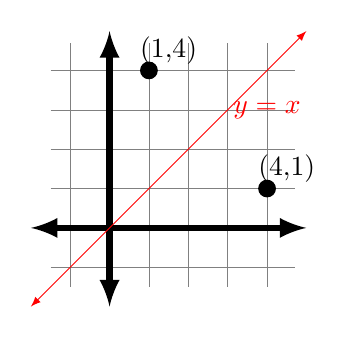
\begin{tikzpicture}[scale=0.5]
            \draw[step=1cm,help lines] (-1.5,-1.5) grid (4.7,4.7);
            \draw[latex-latex, line width=0.08cm] (-2,0) -- (5,0);
            \draw[latex-latex, line width=0.08cm] (0,-2) -- (0,5);
            \draw[latex-latex, color=red, line width=0.01cm] (-2,-2) -- (5,5);
            \node[color=red] at (4,3) {$y=x$};
            \foreach \j/\l in {1/4,4/1}{
                \filldraw [black] (\j,\l) circle [radius=6pt];
                \draw (\j+0.5,\l+0.5) node{(\j,\l)};}
        \end{tikzpicture}
        \caption{Reflexión respecto a la recta $y = x$.}
    \end{figure}

    \item \textbf{Rotación de un ángulo $\theta$ respecto al origen:} \\
    La matriz de rotación de un ángulo $\theta$ es
    \[
    T_{R_\theta} = \begin{pmatrix}
        \cos\theta & -\sin\theta \\
        \sin\theta & \cos\theta
    \end{pmatrix}
    \]
    Por ejemplo, para rotar el punto $(1,4)$ un ángulo $\frac{\pi}{4}$ radianes:
    \[
    \begin{pmatrix}
        \cos\frac{\pi}{4} & -\sin\frac{\pi}{4} \\
        \sin\frac{\pi}{4} & \cos\frac{\pi}{4}
    \end{pmatrix}
    \begin{pmatrix}1\\4\end{pmatrix}
    = \frac{\sqrt{2}}{2} \begin{pmatrix} -3 \\ 5 \end{pmatrix}
    \]
    \begin{figure}[H]\centering
        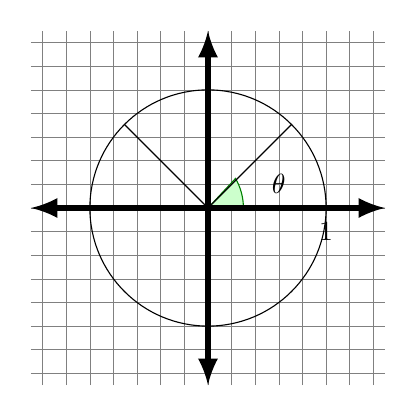
\begin{tikzpicture}[scale=1.5]
            \draw[step=0.2cm,help lines] (-1.5,-1.5) grid (1.5,1.5);
            \filldraw[fill=green!20,draw=green!50!black] (0,0) -- (3mm,0mm) arc [start angle=0, end angle=30, radius=5mm] -- cycle;
            \draw[latex-latex, line width=0.08cm] (-1.5,0)-- (1.5,0);
            \draw[latex-latex, line width=0.08cm] (0,-1.5)-- (0,1.5);
            \draw (0,0) circle [radius=1cm];
            \draw (0.6,0.2) node{$\theta$};
            \draw (1,-0.2) node{1};
            \draw (0,0)-- (0.707106, 0.707106);
            \draw (0,0)-- (-0.707106, 0.707106);
        \end{tikzpicture}
        \caption{Rotación de un punto respecto al origen.}
    \end{figure}

    \item \textbf{Amplificación (escalado) de regiones:} \\
    Suponga que se desea ampliar una figura en el plano un 150\% en el eje $x$ y un 200\% en el eje $y$. Si la transformación lleva el punto $(4,0)$ a $(6,0)$ y $(0,3)$ a $(0,6)$, entonces la matriz de transformación es
    \[
    A = \begin{pmatrix}
        \frac{3}{2} & 0 \\
        0 & 2
    \end{pmatrix}
    \]
    \begin{figure}[H]\centering
        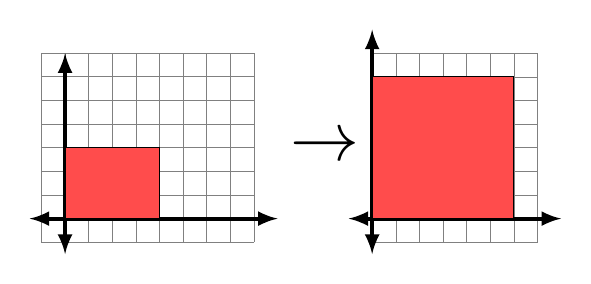
\begin{tikzpicture}[scale=0.3]
            \draw[step=1cm,help lines, line width=0.01cm] (-1,-1) grid (8,7);
            \draw[latex-latex, line width=0.05cm] (-1.5,0) -- (9,0);
            \draw[latex-latex, line width=0.05cm] (0,-1.5) -- (0,7);
            \filldraw[fill=red!70, draw=black] (0,0) rectangle ++(4,3);
            \draw (11,3) node{{\Huge $\to$}};
            \draw[step=1cm,help lines] (13,-1) grid (20,7);
            \draw[latex-latex, line width=0.05cm] (12,0) -- (21,0);
            \draw[latex-latex, line width=0.05cm] (13,-1.5) -- (13,8);
            \filldraw[fill=red!70, draw=black] (13,0) rectangle ++(6,6);
        \end{tikzpicture}
        \caption{Escalado de una región en el plano.}
    \end{figure}
\end{enumerate}

\end{example}


\begin{example}[Transformaciones lineales: la casita y sus imágenes]
Consideremos una figura en el plano (la "casita") representada por los vértices y segmentos en la base canónica de $\mathbb{R}^2$. A continuación se muestran algunos ejemplos de transformaciones lineales aplicadas a esta figura, junto con sus matrices y gráficas.

\begin{enumerate}[(a)]
    \item \textbf{Reflexión respecto al eje $y$:}

    La matriz asociada es
    \[
    A = \begin{pmatrix} -1 & 0 \\ 0 & 1 \end{pmatrix}
    \]
    Esta transformación invierte la coordenada $x$ y deja inalterada la coordenada $y$.

    \begin{figure}[H]\centering
    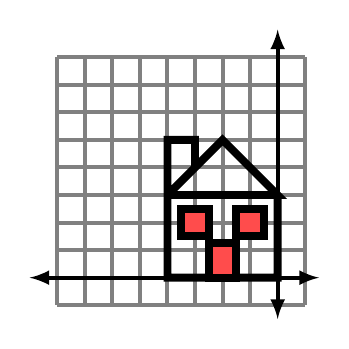
\begin{tikzpicture}[scale=0.35]
        % Ejes y cuadrícula
        \draw[step=1cm,help lines, line width=0.05cm] (1,-1) grid (-8,8);
        \draw[latex-latex, line width=0.05cm] (1.5,0) -- (-9,0);
        \draw[latex-latex, line width=0.05cm] (0,-1.5) -- (0,9);
        % Casita reflejada
        \draw[line width=0.1cm, draw=black] (-3,4)-- (-3,5)-- (-4,5)-- (-4,3)-- (0,3)-- (-2,5)-- (-4,3)-- (-4,0)-- (0,0)-- (0,3);
        \filldraw[line width=0.1cm, fill=red!70, draw=black] (-0.5,1.5) rectangle ++(-1,1);
        \filldraw[line width=0.1cm, fill=red!70, draw=black] (-2.5,1.5) rectangle ++(-1,1);
        \filldraw[line width=0.1cm, fill=red!70, draw=black] (-1.5,0) rectangle ++(-1,1.25);
    \end{tikzpicture}
    \caption{Reflexión de la casita respecto al eje $y$.}
    \end{figure}

    \item \textbf{Dilatación (ampliación) al doble:}

    La matriz asociada es
    \[
    A = \begin{pmatrix} 2 & 0 \\ 0 & 2 \end{pmatrix}
    \]
    Esta transformación multiplica por $2$ cada coordenada, ampliando la figura al doble de su tamaño.

    \begin{figure}[H]\centering
    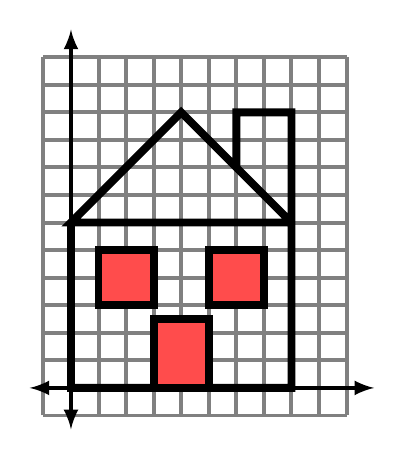
\begin{tikzpicture}[scale=0.35]
        % Ejes y cuadrícula
        \draw[step=1cm,help lines, line width=0.05cm] (-1,-1) grid (10,12);
        \draw[latex-latex, line width=0.05cm] (-1.5,0) -- (11,0);
        \draw[latex-latex, line width=0.05cm] (0,-1.5) -- (0,13);
        % Casita ampliada
        \draw[line width=0.1cm, draw=black] (6,8)-- (6,10)-- (8,10)-- (8,6)-- (0,6)-- (4,10)-- (8,6)-- (8,0)-- (0,0)-- (0,6);
        \filldraw[line width=0.1cm, fill=red!70, draw=black] (1,3) rectangle ++(2,2);
        \filldraw[line width=0.1cm, fill=red!70, draw=black] (5,3) rectangle ++(2,2);
        \filldraw[line width=0.1cm, fill=red!70, draw=black] (3,0) rectangle ++(2,2.5);
    \end{tikzpicture}
    \caption{La casita ampliada al doble.}
    \end{figure}

    \item \textbf{Reflexión respecto al eje $x$:}

    La matriz asociada es
    \[
    A = \begin{pmatrix} 1 & 0 \\ 0 & -1 \end{pmatrix}
    \]
    Esta transformación invierte la coordenada $y$ y deja inalterada la coordenada $x$.

    \begin{figure}[H]\centering
    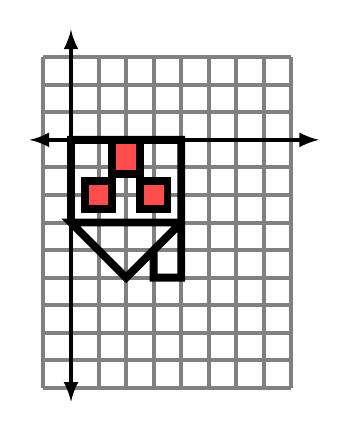
\begin{tikzpicture}[scale=0.35]
        % Ejes y cuadrícula
        \draw[step=1cm,help lines, line width=0.05cm] (-1,-9) grid (8,3);
        \draw[latex-latex, line width=0.05cm] (-1.5,0) -- (9,0);
        \draw[latex-latex, line width=0.05cm] (0,-9.5) -- (0,4);
        % Casita reflejada
        \draw[line width=0.1cm, draw=black] (3,-4)-- (3,-5)-- (4,-5)-- (4,-3)-- (0,-3)-- (2,-5)-- (4,-3)-- (4,0)-- (0,0)-- (0,-3);
        \filldraw[line width=0.1cm, fill=red!70, draw=black] (0.5,-1.5) rectangle ++(1,-1);
        \filldraw[line width=0.1cm, fill=red!70, draw=black] (2.5,-1.5) rectangle ++(1,-1);
        \filldraw[line width=0.1cm, fill=red!70, draw=black] (1.5,0) rectangle ++(1,-1.25);
    \end{tikzpicture}
    \caption{Reflexión de la casita respecto al eje $x$.}
    \end{figure}

\end{enumerate}

\end{example}





\begin{prob}
Sea $S = \{e_1, e_2, e_3\}$ la base canónica de $\mathbb{R}^3$ y sea $B = \{v_1, v_2, v_3\}$ la base que resulta al evaluar los vectores de $S$ en la transformación lineal
\[
T\begin{pmatrix} x_1 \\ x_2 \\ x_3 \end{pmatrix} = \begin{pmatrix} x_1 + x_2 \\ 2x_1 - x_2 + x_3 \\ x_2 + 3x_3 \end{pmatrix}.
\]
Calcule la matriz de cambio de base de la base canónica a la base $B$.
\begin{myproof}
Para obtener la base $B$, aplicamos la transformación $T$ a cada vector de la base canónica $S$:
\[
v_1 = T(e_1) = T\begin{pmatrix}1 \\ 0 \\ 0\end{pmatrix} = \begin{pmatrix}1 + 0 \\ 2 \cdot 1 - 0 + 0 \\ 0 + 3 \cdot 0 \end{pmatrix} = \begin{pmatrix}1 \\ 2 \\ 0 \end{pmatrix},
\]
\[
v_2 = T(e_2) = T\begin{pmatrix}0 \\ 1 \\ 0\end{pmatrix} = \begin{pmatrix}0 + 1 \\ 2 \cdot 0 - 1 + 0 \\ 1 + 3 \cdot 0 \end{pmatrix} = \begin{pmatrix}1 \\ -1 \\ 1 \end{pmatrix},
\]
\[
v_3 = T(e_3) = T\begin{pmatrix}0 \\ 0 \\ 1\end{pmatrix} = \begin{pmatrix}0 + 0 \\ 2 \cdot 0 - 0 + 1 \\ 0 + 3 \cdot 1 \end{pmatrix} = \begin{pmatrix}0 \\ 1 \\ 3 \end{pmatrix}.
\]

La matriz de cambio de base de la base canónica $S$ a la base $B$ está formada por las columnas que son los vectores $v_1, v_2, v_3$ expresados en la base canónica:
\[
P_{S \to B} = \begin{pmatrix}
1 & 1 & 0 \\
2 & -1 & 1 \\
0 & 1 & 3
\end{pmatrix}.
\]
\end{myproof}
\end{prob}


\begin{prob}
Determine si las siguientes funciones son una transformación lineal. Si lo son, use la matriz de representación en las bases canónicas para calcular una base para el kernel y la imagen. Determine el rango y la nulidad de la transformación.

\begin{enumerate}[$a)$]

\item $T:\mathbb{R}^5\rightarrow \mathbb{R}^3$ donde $T\begin{pmatrix}
x_1\\x_2\\x_3\\x_4\\x_5
\end{pmatrix}=\begin{pmatrix}
x_1+x_2\\x_2+x_3+x_4\\x_4+x_5
\end{pmatrix}.$
\begin{myproof}
$T$ es una transformación lineal porque cada componente es una combinación lineal de las variables.

La matriz asociada es:
\[
A = \begin{pmatrix}
1 & 1 & 0 & 0 & 0 \\
0 & 1 & 1 & 1 & 0 \\
0 & 0 & 0 & 1 & 1
\end{pmatrix}
\]

Para el kernel, resolvemos $A\vec{x}=0$:
\[
\begin{cases}
x_1 + x_2 = 0 \\
x_2 + x_3 + x_4 = 0 \\
x_4 + x_5 = 0
\end{cases}
\]
De aquí: $x_1 = -x_2$, $x_4 = -x_5$, $x_3 = -x_2 - x_4 = -x_2 + x_5$.

El kernel es:
\[
\ker(T) = \text{span}\left\{
\begin{pmatrix}-1\\1\\-1\\0\\0\end{pmatrix},
\begin{pmatrix}0\\0\\1\\-1\\1\end{pmatrix}
\right\}
\]
Nulidad $=2$.

Para la imagen, el rango de $A$ es $3$ (las filas son linealmente independientes). Una base para la imagen son las columnas 1, 2 y 4:
\[
\left\{
\begin{pmatrix}1\\0\\0\end{pmatrix},
\begin{pmatrix}1\\1\\0\end{pmatrix},
\begin{pmatrix}0\\1\\1\end{pmatrix}
\right\}
\]
Rango $=3$.
\end{myproof}

\item $T:\mathcal{M}_{2}\left(\mathbb{R}\right) \rightarrow \mathcal{M}_{2}\left(\mathbb{R}\right)$ donde $
T(A)= A^{2}.$
\begin{myproof}
No es una transformación lineal. En general,
\[
T(A+B) = (A+B)^2 = A^2 + AB + BA + B^2 \neq A^2 + B^2 = T(A) + T(B)
\]
Por lo tanto, $T$ no es lineal.
\end{myproof}

\item $T:\mathcal{M}_{2}\left(\mathbb{R}\right) \rightarrow \mathcal{M}_{2}\left(\mathbb{R}\right)$ donde $T(A)=\mathbf{O}_{2\times 2}.$
\begin{myproof}
Sí es lineal porque $T(A+B) = \mathbf{O} = \mathbf{O} + \mathbf{O} = T(A) + T(B)$ y $T(kA) = \mathbf{O} = k\mathbf{O} = kT(A)$.

La matriz asociada es la matriz nula de $4\times 4$. El kernel es todo $\mathcal{M}_2(\mathbb{R})$, con base
\[
\left\{
\begin{pmatrix}1&0\\0&0\end{pmatrix},
\begin{pmatrix}0&1\\0&0\end{pmatrix},
\begin{pmatrix}0&0\\1&0\end{pmatrix},
\begin{pmatrix}0&0\\0&1\end{pmatrix}
\right\}
\]
Nulidad $=4$. Imagen $=\{\mathbf{O}\}$, rango $=0$.
\end{myproof}

\item $T:\mathcal{M}_{2}\left(\mathbb{R}\right) \rightarrow \mathbb{R}$ donde $T\left( \begin{array}{cc} 
	a&b \\
	c&d\\
	\end{array} \right)= 3a-4b+c+d.$
\begin{myproof}
$T$ es lineal, pues es una combinación lineal de las entradas.

La matriz asociada en la base canónica es el vector fila:
\[
A = \begin{pmatrix} 3 & -4 & 1 & 1 \end{pmatrix}
\]
El kernel es el subespacio de matrices $A$ tales que $3a-4b+c+d=0$. Una base se puede obtener resolviendo la ecuación para tres variables libres, por ejemplo:
\[
a = \frac{4}{3}b - \frac{1}{3}c - \frac{1}{3}d
\]
Así, una base del kernel es:
\[
\left\{
\begin{pmatrix}4\\3\\0\\0\end{pmatrix},
\begin{pmatrix}-1\\0\\3\\0\end{pmatrix},
\begin{pmatrix}-1\\0\\0\\3\end{pmatrix}
\right\}
\]
Nulidad $=3$.

La imagen es $\mathbb{R}$, rango $=1$.
\end{myproof}

\item $T:\mathcal{M}_{2}\left(\mathbb{R}\right) \rightarrow \mathcal{M}_{3\times 2}\left(\mathbb{R}\right)$ donde $T\left( \begin{array}{cc} 
	a&b \\
	c&d\\
	\end{array} \right)= \left( \begin{array}{cc} 
	a+b& 2d \\
	2b-d&-3c\\
	2b-c&-3a\\
	\end{array} \right).$
\begin{myproof}
$T$ es lineal, ya que cada entrada es una combinación lineal de $a, b, c, d$.

Si escribimos la matriz como un vector columna:
\[
T\left(\begin{pmatrix}a\\b\\c\\d\end{pmatrix}\right) =
\begin{pmatrix}
a+b \\ 2d \\ 2b-d \\ -3c \\ 2b-c \\ -3a
\end{pmatrix}
\]
La matriz asociada es:
\[
A = \begin{pmatrix}
1 & 1 & 0 & 0 \\
0 & 0 & 0 & 2 \\
0 & 2 & 0 & -1 \\
0 & 0 & -3 & 0 \\
0 & 2 & -1 & 0 \\
-3 & 0 & 0 & 0
\end{pmatrix}
\]
El rango de $A$ es $4$ (por reducción por filas). La nulidad es $0$ (ya que hay 4 columnas y 4 pivotes). El kernel es $\{0\}$ y la imagen es un subespacio de dimensión $4$ en $\mathbb{R}^6$.
\end{myproof}

\item $T:\mathcal{M}_{2}\left(\mathbb{R}\right) \rightarrow \mathcal{P}_{3}(\mathbb{R})$  donde $T\left( \begin{array}{cc} 
	a&b \\
	c&d\\
	\end{array} \right)= 2a+(b-d)x-(a+c)x^2+(a+b-c-d)x^3.$
\begin{myproof}
$T$ es lineal, pues cada coeficiente es una combinación lineal de $a, b, c, d$.

La matriz asociada en las bases canónicas es:
\[
A = \begin{pmatrix}
2 & 0 & 0 & 0 \\
0 & 1 & 0 & -1 \\
-1 & 0 & -1 & 0 \\
1 & 1 & -1 & -1
\end{pmatrix}
\]
El rango es $4$ (matriz cuadrada e invertible), nulidad $=0$. El kernel es $\{0\}$, la imagen es todo $\mathcal{P}_3(\mathbb{R})$.
\end{myproof}

\item $T:\mathcal{P}_{2}(\mathbb{R}) \rightarrow \mathcal{P}_{2}(\mathbb{R})$ donde $T(a_0+a_1x+a_2x^2)= a_0+a_1(x+1)+a_2(x+1)^2.$
\begin{myproof}
$T$ es lineal, pues es una combinación lineal de los coeficientes.

Calculando la imagen de la base estándar:
\[
T(1) = 1, \quad T(x) = x+1, \quad T(x^2) = (x+1)^2 = x^2 + 2x + 1
\]
Expresando en la base $\{1, x, x^2\}$:
\[
T(1) = (1, 0, 0), \quad T(x) = (1, 1, 0), \quad T(x^2) = (1, 2, 1)
\]
La matriz asociada es:
\[
A = \begin{pmatrix}
1 & 1 & 1 \\
0 & 1 & 2 \\
0 & 0 & 1
\end{pmatrix}
\]
$\det(A) = 1 \neq 0$ así que $A$ es invertible, el kernel es $\{0\}$, la imagen es todo $\mathcal{P}_2(\mathbb{R})$, rango $=3$, nulidad $=0$.
\end{myproof}

\item $T:\mathcal{P}_{2}(\mathbb{R}) \rightarrow \mathcal{P}_{2}(\mathbb{R})$ donde $T(a_0+a_1x+a_2x^2)=(a_0+1)+(a_1+1)x+(a_2+1)x^2.$
\begin{myproof}
No es lineal, pues $T(0) = 1 + 1x + 1x^2 \neq 0$ y tampoco se cumple la aditividad ni la homogeneidad.
\end{myproof}

\item $T:\mathcal{P}_{3}(\mathbb{R}) \rightarrow \mathcal{P}_{2}(\mathbb{R})$ donde $T(a_0+a_1x+a_2x^2+a_3x^3)= 5a_0-7a_3x^2.$
\begin{myproof}
$T$ es lineal. La matriz asociada en bases canónicas es:
\[
A = \begin{pmatrix}
5 & 0 & 0 & 0 \\
0 & 0 & 0 & 0 \\
0 & 0 & 0 & -7
\end{pmatrix}
\]
El kernel es el subespacio generado por $x$ y $x^2$, es decir, $\text{span}\{x, x^2\}$. Nulidad $=2$. La imagen es $\text{span}\{1, x^2\}$, rango $=2$.
\end{myproof}

\item $T:\mathcal{P}_{2}(\mathbb{R}) \rightarrow \mathcal{P}_{3}(\mathbb{R})$ donde $T(p(x))=xp(x).$
\begin{myproof}
$T$ es lineal. En la base $\{1, x, x^2\}$ de $\mathcal{P}_2(\mathbb{R})$ y $\{1, x, x^2, x^3\}$ de $\mathcal{P}_3(\mathbb{R})$:
\[
T(1) = x, \quad T(x) = x^2, \quad T(x^2) = x^3
\]
La matriz asociada es:
\[
A = \begin{pmatrix}
0 & 0 & 0 \\
1 & 0 & 0 \\
0 & 1 & 0 \\
0 & 0 & 1
\end{pmatrix}
\]
El kernel es $\{0\}$, rango $=3$, nulidad $=0$. La imagen es $\text{span}\{x, x^2, x^3\}$.
\end{myproof}

\item $T:\mathcal{P}_{2}(\mathbb{R}) \rightarrow \mathcal{P}_{1}(\mathbb{R})$ donde $T(a_0+a_1x+a_2x^2) =(a_0+a_1)-(2a_1+3a_2)x.$
\begin{myproof}
$T$ es lineal. En la base estándar:
\[
T(1) = 1, \quad T(x) = 1 - 2x, \quad T(x^2) = -3x
\]
Matriz asociada:
\[
A = \begin{pmatrix}
1 & 1 & 0 \\
0 & -2 & -3
\end{pmatrix}
\]
Rango $=2$, nulidad $=1$. El kernel es generado por $(1, -1, 1)$, es decir, $1 - x + x^2$.
\end{myproof}

\item $T:\mathcal{P}_{2}(\mathbb{R}) \rightarrow \mathcal{P}_{3}(\mathbb{R})$ donde $T(c_0+c_1x+c_2x^2)=x(c_0+c_1(x-3)+c_2(x-3)^2).$
\begin{myproof}
$T$ es lineal. Expandiendo:
\[
T(c_0+c_1x+c_2x^2) = x\left[c_0 + c_1(x-3) + c_2(x^2 - 6x + 9)\right]
\]
\[
= x[c_0 + c_1x - 3c_1 + c_2x^2 - 6c_2x + 9c_2]
\]
\[
= c_0 x + c_1 x^2 - 3c_1 x + c_2 x^3 - 6c_2 x^2 + 9c_2 x
\]
\[
= (c_0 - 3c_1 + 9c_2)x + (c_1 - 6c_2)x^2 + c_2 x^3
\]
La matriz asociada es:
\[
A = \begin{pmatrix}
0 & 0 & 0 \\
c_0 - 3c_1 + 9c_2 & c_1 - 6c_2 & c_2
\end{pmatrix}
\]
Expresando los coeficientes en la base estándar, se obtiene:
\[
A = \begin{pmatrix}
0 & 0 & 0 \\
1 & -3 & 9 \\
0 & 1 & -6 \\
0 & 0 & 1
\end{pmatrix}
\]
El rango es $3$, nulidad $=0$. El kernel es $\{0\}$.
\end{myproof}

\end{enumerate}
\end{prob}


\begin{prob}
Sea $D:\mathcal{P}_{2}(\mathbb{R}) \rightarrow \mathcal{P}_{2}(\mathbb{R})$ el operador derivada $D(p(x))=p^{\prime}(x).$ Encuentre la matriz $D$ relativa a la base $B=\left\lbrace 1,x,x^2  \right\rbrace.$ Use $D$ para calcular $D(6-6x+24x^2).$
\begin{myproof}
Para encontrar la matriz de $D$ relativa a la base $B = \{1, x, x^2\}$, derivamos cada elemento de la base y expresamos el resultado en términos de $B$:
\[
\begin{aligned}
D(1) &= 0 = 0\cdot 1 + 0\cdot x + 0\cdot x^2 \\
D(x) &= 1 = 1\cdot 1 + 0\cdot x + 0\cdot x^2 \\
D(x^2) &= 2x = 0\cdot 1 + 2\cdot x + 0\cdot x^2
\end{aligned}
\]
Por lo tanto, la matriz asociada es:
\[
[D]_B = \begin{pmatrix}
0 & 1 & 0 \\
0 & 0 & 2 \\
0 & 0 & 0
\end{pmatrix}
\]

Para calcular $D(6 - 6x + 24x^2)$, primero escribimos el vector de coordenadas respecto a $B$:
\[
\vec{p} = \begin{pmatrix} 6 \\ -6 \\ 24 \end{pmatrix}
\]
Multiplicamos por la matriz $[D]_B$:
\[
[D]_B \cdot \vec{p} = 
\begin{pmatrix}
0 & 1 & 0 \\
0 & 0 & 2 \\
0 & 0 & 0
\end{pmatrix}
\begin{pmatrix} 6 \\ -6 \\ 24 \end{pmatrix}
=
\begin{pmatrix}
0 \cdot 6 + 1 \cdot (-6) + 0 \cdot 24 \\
0 \cdot 6 + 0 \cdot (-6) + 2 \cdot 24 \\
0
\end{pmatrix}
=
\begin{pmatrix}
-6 \\ 48 \\ 0
\end{pmatrix}
\]
Por lo tanto,
\[
D(6 - 6x + 24x^2) = -6 + 48x
\]
\end{myproof}
\end{prob}

\begin{prob}
Defina $T: \mathbb{R}^2 \rightarrow \mathbb{R}^3$ como
\[
T\begin{pmatrix}
 x_1\\x_2
\end{pmatrix}=\begin{pmatrix}
x_1+2x_2 \\
	-x_1 \\
	0\\
\end{pmatrix}.
\]
Calcule la matriz de representación de la transformación lineal donde $B=\left\lbrace \begin{pmatrix} 1 \\ 3 \end{pmatrix}, \begin{pmatrix} -2 \\ 4 \end{pmatrix} \right\rbrace$ es la base del espacio de salida y $B'=\left\lbrace \begin{pmatrix} 1 \\ 1 \\ 1 \end{pmatrix}, \begin{pmatrix} 2 \\ 2 \\ 0 \end{pmatrix}, \begin{pmatrix} 3 \\ 0 \\ 0 \end{pmatrix} \right\rbrace$ es base del espacio de llegada. Calcule una base para el kernel y la imagen de $T$.
\begin{myproof}
\textbf{Matriz de representación en las bases dadas:}

Primero, escribimos los vectores de la base $B$ del dominio:
\[
v_1 = \begin{pmatrix} 1 \\ 3 \end{pmatrix}, \quad v_2 = \begin{pmatrix} -2 \\ 4 \end{pmatrix}
\]

Calculamos sus imágenes por $T$:
\[
T(v_1) = T\begin{pmatrix} 1 \\ 3 \end{pmatrix} = \begin{pmatrix} 1 + 2 \cdot 3 \\ -1 \\ 0 \end{pmatrix} = \begin{pmatrix} 7 \\ -1 \\ 0 \end{pmatrix}
\]
\[
T(v_2) = T\begin{pmatrix} -2 \\ 4 \end{pmatrix} = \begin{pmatrix} -2 + 2 \cdot 4 \\ 2 \\ 0 \end{pmatrix} = \begin{pmatrix} 6 \\ 2 \\ 0 \end{pmatrix}
\]

Ahora, expresamos $T(v_1)$ y $T(v_2)$ en la base $B'$ del codominio. Buscamos escalares $a_1, a_2, a_3$ tales que:
\[
T(v_1) = a_1 \begin{pmatrix} 1 \\ 1 \\ 1 \end{pmatrix} + a_2 \begin{pmatrix} 2 \\ 2 \\ 0 \end{pmatrix} + a_3 \begin{pmatrix} 3 \\ 0 \\ 0 \end{pmatrix}
\]
\[
\begin{pmatrix} 7 \\ -1 \\ 0 \end{pmatrix} = a_1 \begin{pmatrix} 1 \\ 1 \\ 1 \end{pmatrix} + a_2 \begin{pmatrix} 2 \\ 2 \\ 0 \end{pmatrix} + a_3 \begin{pmatrix} 3 \\ 0 \\ 0 \end{pmatrix}
\]
Esto da el sistema:
\[
\begin{cases}
7 = a_1 + 2a_2 + 3a_3 \\
-1 = a_1 + 2a_2 \\
0 = a_1
\end{cases}
\implies a_1 = 0,\ -1 = 2a_2 \implies a_2 = -\frac{1}{2},\ 7 = 2(-\frac{1}{2}) + 3a_3 \implies 7 = -1 + 3a_3 \implies a_3 = \frac{8}{3}
\]
Por lo tanto,
\[
[T(v_1)]_{B'} = \begin{pmatrix} 0 \\ -\frac{1}{2} \\ \frac{8}{3} \end{pmatrix}
\]

De igual modo, para $T(v_2)$:
\[
\begin{pmatrix} 6 \\ 2 \\ 0 \end{pmatrix} = b_1 \begin{pmatrix} 1 \\ 1 \\ 1 \end{pmatrix} + b_2 \begin{pmatrix} 2 \\ 2 \\ 0 \end{pmatrix} + b_3 \begin{pmatrix} 3 \\ 0 \\ 0 \end{pmatrix}
\]
\[
\begin{cases}
6 = b_1 + 2b_2 + 3b_3 \\
2 = b_1 + 2b_2 \\
0 = b_1
\end{cases}
\implies b_1 = 0,\ 2 = 2b_2 \implies b_2 = 1,\ 6 = 2(1) + 3b_3 \implies 6 = 2 + 3b_3 \implies b_3 = \frac{4}{3}
\]
Por lo tanto,
\[
[T(v_2)]_{B'} = \begin{pmatrix} 0 \\ 1 \\ \frac{4}{3} \end{pmatrix}
\]

La matriz de representación de $T$ en las bases $B$ y $B'$ es:
\[
[T]_{B',B} = \begin{pmatrix}
0 & 0 \\
-\frac{1}{2} & 1 \\
\frac{8}{3} & \frac{4}{3}
\end{pmatrix}
\]

\textbf{Base para el kernel y la imagen de $T$:}

La matriz de $T$ en las bases canónicas es:
\[
A = \begin{pmatrix}
1 & 2 \\
-1 & 0 \\
0 & 0
\end{pmatrix}
\]
Resolvemos $A\begin{pmatrix}x_1\\x_2\end{pmatrix} = 0$:
\[
\begin{cases}
x_1 + 2x_2 = 0 \\
-x_1 = 0 \\
0 = 0
\end{cases}
\implies x_1 = 0,\ 2x_2 = 0 \implies x_2 = 0
\]
Por lo tanto, $\ker(T) = \{0\}$.

La imagen de $T$ es el subespacio generado por las columnas de $A$:
\[
\text{Im}(T) = \text{span}\left\{ \begin{pmatrix}1\\-1\\0\end{pmatrix}, \begin{pmatrix}2\\0\\0\end{pmatrix} \right\}
\]
Estas dos columnas son linealmente independientes, así que una base para la imagen de $T$ es:
\[
\left\{ \begin{pmatrix}1\\-1\\0\end{pmatrix},\ \begin{pmatrix}2\\0\\0\end{pmatrix} \right\}
\]
\end{myproof}
\end{prob}


\begin{prob}
Sea $A = \begin{pmatrix}
3 & -2 & 1 & 0 \\
1 & 6 & 2 & 1 \\
-3 & 0 & 7 & 1
\end{pmatrix}$ la matriz de representación de una transformación lineal $T: \mathbb{R}^4 \rightarrow \mathbb{R}^3$ en las bases canónicas. Sea
\[
B = \left\lbrace
\begin{pmatrix} 0 \\ 1 \\ 1 \\ 1 \end{pmatrix},
\begin{pmatrix} 2 \\ 1 \\ -1 \\ -1 \end{pmatrix},
\begin{pmatrix} 1 \\ 4 \\ -1 \\ 2 \end{pmatrix},
\begin{pmatrix} 6 \\ 9 \\ 4 \\ 0 \end{pmatrix}
\right\rbrace
\]
una base del dominio y
\[
B' = \left\lbrace
\begin{pmatrix} 0 \\ 8 \\ 8 \end{pmatrix},
\begin{pmatrix} -7 \\ 8 \\ 1 \end{pmatrix},
\begin{pmatrix} -6 \\ 9 \\ 1 \end{pmatrix}
\right\rbrace
\]
una base del codominio. Calcule $T\left(\begin{pmatrix} x_1 \\ x_2 \\ x_3 \\ x_4 \end{pmatrix}\right)$ y exprese el resultado en coordenadas respecto a la base $B'$.
\begin{myproof}
Primero, calculamos $T\left(\begin{pmatrix} x_1 \\ x_2 \\ x_3 \\ x_4 \end{pmatrix}\right)$ en la base canónica:
\[
T\left(\begin{pmatrix} x_1 \\ x_2 \\ x_3 \\ x_4 \end{pmatrix}\right) = A \begin{pmatrix} x_1 \\ x_2 \\ x_3 \\ x_4 \end{pmatrix}
= \begin{pmatrix}
3x_1 - 2x_2 + x_3 \\
x_1 + 6x_2 + 2x_3 + x_4 \\
-3x_1 + 7x_3 + x_4
\end{pmatrix}
\]

Para expresar este vector en la base $B'$, buscamos los escalares $c_1, c_2, c_3$ tales que:
\[
T\left(\begin{pmatrix} x_1 \\ x_2 \\ x_3 \\ x_4 \end{pmatrix}\right) = c_1 \begin{pmatrix} 0 \\ 8 \\ 8 \end{pmatrix} + c_2 \begin{pmatrix} -7 \\ 8 \\ 1 \end{pmatrix} + c_3 \begin{pmatrix} -6 \\ 9 \\ 1 \end{pmatrix}
\]
Esto equivale a resolver el sistema lineal $B' \cdot \vec{c} = T(x)$, donde $B'$ es la matriz cuyas columnas son los vectores de la base $B'$.

Calculando explícitamente:
\[
\begin{pmatrix}
c_1 \\
c_2 \\
c_3
\end{pmatrix}
=
(B')^{-1} \cdot T\left(\begin{pmatrix} x_1 \\ x_2 \\ x_3 \\ x_4 \end{pmatrix}\right)
\]

El resultado es:
\[
\begin{pmatrix}
-\frac{43}{112}x_1 - \frac{1}{14}x_2 + \frac{13}{14}x_3 + \frac{1}{8}x_4 \\
-\frac{24}{7}x_1 - \frac{10}{7}x_2 + \frac{11}{7}x_3 \\
\frac{7}{2}x_1 + 2x_2 - 2x_3
\end{pmatrix}
\]

Por lo tanto,
\[
T\left(\begin{pmatrix} x_1 \\ x_2 \\ x_3 \\ x_4 \end{pmatrix}\right)_{B'} =
\begin{pmatrix}
-\frac{43}{112}x_1 - \frac{1}{14}x_2 + \frac{13}{14}x_3 + \frac{1}{8}x_4 \\
-\frac{24}{7}x_1 - \frac{10}{7}x_2 + \frac{11}{7}x_3 \\
\frac{7}{2}x_1 + 2x_2 - 2x_3
\end{pmatrix}_{B'}
\]
\end{myproof}
\end{prob}

 
\begin{prob}
Sea $A = \begin{pmatrix}
0 & 1 & 0 \\
1 & 0 & 0 \\
0 & 0 & 0
\end{pmatrix}$. Demuestre que, en relación al espacio con coordenadas $XYZ$, el espacio nulo de $A$ consiste en todos los puntos del plano $Z$ y que el espacio columna consiste en todos los puntos del plano $XY$.
\begin{myproof}
El \textbf{espacio nulo} (o kernel) de $A$ es el conjunto de vectores $v = (x, y, z)^T$ tales que $A v = 0$:
\[
A \begin{pmatrix} x \\ y \\ z \end{pmatrix} = \begin{pmatrix} y \\ x \\ 0 \end{pmatrix} = \begin{pmatrix} 0 \\ 0 \\ 0 \end{pmatrix}
\]
Esto implica $x = 0$ y $y = 0$, pero $z$ es libre. Por lo tanto,
\[
\ker(A) = \left\{ \begin{pmatrix} 0 \\ 0 \\ z \end{pmatrix} : z \in \mathbb{R} \right\}
\]
Esto corresponde exactamente al eje $Z$, es decir, a todos los puntos del plano $Z$ (el subespacio generado por el vector $(0,0,1)$).

El \textbf{espacio columna} de $A$ es el subespacio generado por sus columnas:
\[
\text{Col}(A) = \text{span}\left\{ \begin{pmatrix} 0 \\ 1 \\ 0 \end{pmatrix}, \begin{pmatrix} 1 \\ 0 \\ 0 \end{pmatrix}, \begin{pmatrix} 0 \\ 0 \\ 0 \end{pmatrix} \right\}
\]
Las dos primeras columnas son linealmente independientes y generan el plano $XY$, es decir,
\[
\text{Col}(A) = \left\{ \begin{pmatrix} a \\ b \\ 0 \end{pmatrix} : a, b \in \mathbb{R} \right\}
\]
Por lo tanto, el espacio columna de $A$ consiste en todos los puntos del plano $XY$.

Esto coincide con los resultados computacionales: el núcleo es generado por $(0,0,1)$ y el espacio columna por $(1,0,0)$ y $(0,1,0)$.
\end{myproof}
\end{prob}


\begin{prob}
Encuentre una matriz $3\times 3$ cuyo espacio nulo sea el eje $X$ y cuyo espacio columna sea el plano $YZ$.
\begin{myproof}
Queremos que el espacio nulo (kernel) sea el eje $X$, es decir, todos los vectores de la forma $(x,0,0)^T$. Esto implica que la matriz $A$ debe anular cualquier vector cuya única componente no nula sea la primera.

Además, queremos que el espacio columna (imagen) de $A$ sea el plano $YZ$, es decir, todos los vectores de la forma $(0, y, z)^T$. Esto significa que las columnas de $A$ deben generar el subespacio $YZ$ y, por lo tanto, su primera fila debe ser toda cero.

Una matriz que cumple estas condiciones es:
\[
A = \begin{pmatrix}
0 & 0 & 0 \\
0 & 1 & 0 \\
0 & 0 & 1
\end{pmatrix}
\]

Verificación:
\begin{itemize}
    \item \textbf{Espacio nulo:} $A\begin{pmatrix} x \\ 0 \\ 0 \end{pmatrix} = \begin{pmatrix} 0 \\ 0 \\ 0 \end{pmatrix}$ para cualquier $x$. Si $A\begin{pmatrix} x \\ y \\ z \end{pmatrix} = 0$, entonces $y = 0$ y $z = 0$, así que el núcleo es exactamente el eje $X$.
    \item \textbf{Espacio columna:} Las columnas de $A$ son $\begin{pmatrix} 0 \\ 0 \\ 0 \end{pmatrix}$, $\begin{pmatrix} 0 \\ 1 \\ 0 \end{pmatrix}$ y $\begin{pmatrix} 0 \\ 0 \\ 1 \end{pmatrix}$, que generan el plano $YZ$.
\end{itemize}
\end{myproof}
\end{prob}




\begin{prob}
Sea $V$ un espacio vectorial de dimensión $m$. Demuestre que si $T:V\rightarrow \mathbb{R}^n$ es una transformación lineal inyectiva y $\left\lbrace v_1,v_2,\dots , v_k \right\rbrace$ con $k\leq m$ es un conjunto linealmente independiente en $V$, entonces $\left\lbrace T(v_1), T(v_2), \dots , T(v_k)  \right\rbrace$ es un conjunto linealmente independiente en $\mathbb{R}^n$.
\begin{myproof}
Sea $T: V \to \mathbb{R}^n$ una transformación lineal inyectiva y sea $\{v_1, v_2, \dots, v_k\}$ un conjunto linealmente independiente en $V$ con $k \leq m = \dim(V)$.

Supongamos que existen escalares $a_1, a_2, \dots, a_k$ tales que
\[
    a_1 T(v_1) + a_2 T(v_2) + \cdots + a_k T(v_k) = 0.
\]
Por la linealidad de $T$, esto implica
\[
    T(a_1 v_1 + a_2 v_2 + \cdots + a_k v_k) = 0.
\]
Como $T$ es inyectiva, su núcleo es trivial, es decir,
\[
    a_1 v_1 + a_2 v_2 + \cdots + a_k v_k = 0.
\]
Dado que $\{v_1, v_2, \dots, v_k\}$ es linealmente independiente, se concluye que
\[
    a_1 = a_2 = \cdots = a_k = 0.
\]
Por lo tanto, $\{T(v_1), T(v_2), \dots, T(v_k)\}$ es un conjunto linealmente independiente en $\mathbb{R}^n$.
\end{myproof}
\end{prob}

\begin{prob}
Sea $V$ un espacio vectorial de dimensión $m$. Demuestre que si $T:V\rightarrow \mathbb{R}^n$ es una transformación lineal y $\left\lbrace v_1,v_2,\dots , v_k \right\rbrace$ con $k\leq m$ es un conjunto linealmente dependiente en $V$, entonces $\left\lbrace T(v_1), T(v_2), \dots , T(v_k)  \right\rbrace$ es un conjunto linealmente dependiente en $\mathbb{R}^n$.
\begin{myproof}
Sea $T: V \to \mathbb{R}^n$ una transformación lineal y sea $\{v_1, v_2, \dots, v_k\}$ un conjunto linealmente dependiente en $V$ con $k \leq m = \dim(V)$.

Por definición de dependencia lineal, existen escalares no todos cero $a_1, a_2, \dots, a_k$ tales que
\[
    a_1 v_1 + a_2 v_2 + \cdots + a_k v_k = 0.
\]
Aplicando la transformación lineal $T$ y usando su linealidad, se tiene
\[
    a_1 T(v_1) + a_2 T(v_2) + \cdots + a_k T(v_k) = T(0) = 0.
\]
Por lo tanto, $\{T(v_1), T(v_2), \dots, T(v_k)\}$ es un conjunto linealmente dependiente en $\mathbb{R}^n$.
\end{myproof}
\end{prob}




\begin{prob}
Sea $T: V \rightarrow W$ una transformación lineal. Demuestre que si $\{v_1, v_2, \dots, v_n\}$ es una base de $V$ y $\{v_1, v_2, \dots, v_k\}$ es una base de $\ker(T)$, entonces 
\[
\{T(v_{k+1}), T(v_{k+2}), \dots, T(v_n)\}
\]
es una base de $\operatorname{Im}(T)$.
\begin{myproof}
Como $\{v_1, \dots, v_n\}$ es base de $V$, todo vector $v \in V$ se puede escribir de forma única como
\[
v = \sum_{i=1}^n a_i v_i.
\]
Aplicando $T$, obtenemos
\[
T(v) = \sum_{i=1}^n a_i T(v_i) = \sum_{i=k+1}^n a_i T(v_i),
\]
ya que para $1 \leq i \leq k$, $v_i \in \ker(T)$ implica que $T(v_i) = 0$.

Por lo tanto, $\operatorname{Im}(T)$ está generado por $\{T(v_{k+1}), \dots, T(v_n)\}$.

Para demostrar que este conjunto es linealmente independiente, supongamos que existen escalares $c_{k+1}, \dots, c_n$ tales que
\[
\sum_{i=k+1}^n c_i T(v_i) = 0.
\]
Esto implica que
\[
T\left(\sum_{i=k+1}^n c_i v_i\right) = 0,
\]
es decir, $\sum_{i=k+1}^n c_i v_i \in \ker(T)$.

Pero como $\{v_1, \dots, v_k\}$ es base de $\ker(T)$ y $\{v_1, \dots, v_n\}$ es base de $V$, la expresión
\[
\sum_{i=k+1}^n c_i v_i = \sum_{j=1}^k d_j v_j
\]
para algunos escalares $d_j$.

Reordenando,
\[
\sum_{j=1}^k (-d_j) v_j + \sum_{i=k+1}^n c_i v_i = 0.
\]
Dado que $\{v_1, \dots, v_n\}$ es base, todos los coeficientes deben ser cero, por lo que
\[
c_i = 0 \quad \text{para } i = k+1, \dots, n.
\]

Por lo tanto, $\{T(v_{k+1}), \dots, T(v_n)\}$ es linealmente independiente y, junto con la generación demostrada, es base de $\operatorname{Im}(T)$.
\end{myproof}
\end{prob}


\begin{prob}
Sea $A$ una matriz $m\times n$. Demuestre el teorema de la dimensión para matrices, es decir, demuestre que $\mathrm{nulidad}(A) + \mathrm{rango}(A) = n$.
\begin{myproof}
El teorema de la dimensión para matrices, también conocido como teorema rango-nulidad, afirma que para cualquier matriz $A$ de tamaño $m \times n$:
\[
\mathrm{nulidad}(A) + \mathrm{rango}(A) = n,
\]
donde $\mathrm{rango}(A)$ es la dimensión del espacio columna de $A$ (el número de columnas linealmente independientes) y $\mathrm{nulidad}(A)$ es la dimensión del espacio nulo de $A$ (el conjunto de soluciones de $A\vec{x} = 0$).

\textbf{Demostración:}

Al reducir $A$ a su forma escalonada por filas, el número de columnas con pivote (unos principales) es igual al rango $r$ de $A$. Las variables asociadas a columnas sin pivote son variables libres, y su número es $n - r$.

Cada variable libre corresponde a un vector linealmente independiente en el espacio nulo, por lo que la nulidad de $A$ es precisamente el número de variables libres:
\[
\mathrm{nulidad}(A) = n - \mathrm{rango}(A).
\]
Reordenando,
\[
\mathrm{nulidad}(A) + \mathrm{rango}(A) = n.
\]

De manera formal, si $A$ define una transformación lineal $T: \mathbb{R}^n \to \mathbb{R}^m$, entonces el teorema rango-nulidad se deduce del hecho de que la dimensión del dominio es igual a la suma de la dimensión del núcleo y la dimensión de la imagen:
\[
\dim(\ker T) + \dim(\operatorname{Im} T) = \dim(\mathbb{R}^n) = n.
\]

Por lo tanto, para cualquier matriz $A$ de tamaño $m \times n$,
\[
\mathrm{nulidad}(A) + \mathrm{rango}(A) = n.
\]
\end{myproof}
\end{prob}




\begin{prob}
Defina $W = \operatorname{span}\{1, \sin x, \cos x\}$ como subespacio de $\mathcal{C}[0,2\pi]$ y sea $T: W \rightarrow \mathbb{R}^3$ la transformación lineal $T(f(x)) = \begin{pmatrix} 0 \\ \pi \\ 2\pi \end{pmatrix}$. Calcule:

\begin{enumerate}[$a)$]
\item $T(1 + \sin x + \cos x)$.
\begin{myproof}
Por la definición de $T$, para cualquier $f(x) \in W$, $T(f(x)) = \begin{pmatrix} 0 \\ \pi \\ 2\pi \end{pmatrix}$, independientemente de $f(x)$. Por lo tanto,
\[
T(1 + \sin x + \cos x) = \begin{pmatrix} 0 \\ \pi \\ 2\pi \end{pmatrix}.
\]
\end{myproof}

\item La matriz de representación de $T$ respecto a la base $\{1, \sin x, \cos x\}$ de $W$.
\begin{myproof}
La base de $W$ es $\{1, \sin x, \cos x\}$. Calculamos la imagen de cada vector base:
\[
T(1) = T(\sin x) = T(\cos x) = \begin{pmatrix} 0 \\ \pi \\ 2\pi \end{pmatrix}.
\]
Por lo tanto, la matriz asociada es:
\[
A = \begin{pmatrix}
0 & 0 & 0 \\
\pi & \pi & \pi \\
2\pi & 2\pi & 2\pi
\end{pmatrix}
\]
\end{myproof}

\item Una base para el kernel de $T$.
\begin{myproof}
El kernel de $T$ es el conjunto de $f(x) = a_1 \cdot 1 + a_2 \sin x + a_3 \cos x$ tal que $T(f(x)) = 0$, es decir,
\[
\begin{pmatrix}
0 \\ \pi \\ 2\pi
\end{pmatrix} = 0 \implies \pi = 0,\, 2\pi = 0,
\]
lo cual nunca ocurre para valores reales de $\pi$. Sin embargo, dado que la imagen de cualquier $f(x)$ es siempre el vector fijo, el kernel es el subespacio de $W$ formado por todos los $f(x)$ tales que $T(f(x)) = 0$, pero como $T$ nunca es cero salvo para el vector nulo, el kernel es $\{0\}$.

Por lo tanto, una base para el kernel es $\emptyset$ o $\{0\}$.
\end{myproof}

\item Una base para la imagen de $T$.
\begin{myproof}
La imagen de $T$ es el subespacio de $\mathbb{R}^3$ generado por el vector $\begin{pmatrix} 0 \\ \pi \\ 2\pi \end{pmatrix}$. Por lo tanto, una base para la imagen es:
\[
\left\{ \begin{pmatrix} 0 \\ \pi \\ 2\pi \end{pmatrix} \right\}
\]
\end{myproof}
\end{enumerate}
\end{prob}


\begin{prob}
Defina $W := \left\lbrace f \in \mathcal{C}\left[ -1,1 \right] \mid f(0) = 0 \right\rbrace$ y $T: \mathcal{C}\left[ -1,1 \right] \rightarrow W$ como $T(f(x)) = f(x) - f(0)$. Determine si $T$ es una transformación lineal y, si lo es, calcule una base para el kernel y la imagen de $T$.
\begin{myproof}
\textbf{Linealidad:}  
Sea $f, g \in \mathcal{C}[-1,1]$ y $k \in \mathbb{R}$.  
\[
T(f+g)(x) = (f+g)(x) - (f+g)(0) = f(x) + g(x) - f(0) - g(0) = (f(x) - f(0)) + (g(x) - g(0)) = T(f)(x) + T(g)(x)
\]
\[
T(kf)(x) = (kf)(x) - (kf)(0) = kf(x) - kf(0) = k(f(x) - f(0)) = kT(f)(x)
\]
Por lo tanto, $T$ es una transformación lineal.

\textbf{Kernel de $T$:}  
Buscamos todas las $f$ tales que $T(f) = 0$, es decir,
\[
f(x) - f(0) = 0 \implies f(x) = f(0)\ \forall x
\]
Por lo tanto, el kernel está formado por todas las funciones constantes. Una base para el kernel es la función constante $1$.

\textbf{Imagen de $T$:}  
Para cualquier $f \in \mathcal{C}[-1,1]$, $T(f)(0) = f(0) - f(0) = 0$. Por lo tanto, la imagen de $T$ es el subespacio $W = \{g \in \mathcal{C}[-1,1] \mid g(0) = 0\}$, es decir, el conjunto de funciones continuas que se anulan en $0$. Este subespacio es de dimensión infinita y no admite una base finita, pero puede describirse simplemente como $W$.
\end{myproof}
\end{prob}


\begin{prob}
Defina $T: \mathbb{R}^2 \rightarrow \mathbb{R}^3$ la transformación lineal tal que
\[
T\begin{pmatrix} 3 \\ 2 \end{pmatrix} = \begin{pmatrix} 1 \\ 2 \\ 3 \end{pmatrix}, \qquad
T\begin{pmatrix} 4 \\ 3 \end{pmatrix} = \begin{pmatrix} 0 \\ -5 \\ 1 \end{pmatrix}.
\]
Calcule la matriz de representación de $T$ respecto a la base canónica de $\mathbb{R}^2$ y determine el rango y la nulidad de $T$.
\begin{myproof}
Sea $e_1 = \begin{pmatrix} 1 \\ 0 \end{pmatrix}$ y $e_2 = \begin{pmatrix} 0 \\ 1 \end{pmatrix}$ la base canónica de $\mathbb{R}^2$. Queremos encontrar $T(e_1)$ y $T(e_2)$.

Expresamos los vectores dados en términos de $e_1$ y $e_2$:
\[
\begin{pmatrix} 3 \\ 2 \end{pmatrix} = 3e_1 + 2e_2, \quad
\begin{pmatrix} 4 \\ 3 \end{pmatrix} = 4e_1 + 3e_2.
\]

Sea $T(e_1) = \begin{pmatrix} a_1 \\ a_2 \\ a_3 \end{pmatrix}$ y $T(e_2) = \begin{pmatrix} b_1 \\ b_2 \\ b_3 \end{pmatrix}$. Entonces:
\[
3T(e_1) + 2T(e_2) = \begin{pmatrix} 1 \\ 2 \\ 3 \end{pmatrix}
\]
\[
4T(e_1) + 3T(e_2) = \begin{pmatrix} 0 \\ -5 \\ 1 \end{pmatrix}
\]

Esto nos da, para cada componente $i$:
\[
\begin{cases}
3a_i + 2b_i = u_i \\
4a_i + 3b_i = v_i
\end{cases}
\]
donde $u = (1,2,3)^T$, $v = (0,-5,1)^T$.

Resolviendo para cada componente:

\textbf{Primera componente:}
\[
\begin{cases}
3a_1 + 2b_1 = 1 \\
4a_1 + 3b_1 = 0
\end{cases}
\]
Multiplicamos la primera ecuación por $3$ y la segunda por $-2$ y sumamos:
\[
9a_1 + 6b_1 = 3 \\
-8a_1 - 6b_1 = 0 \\
a_1 = 3
\]
Sustituyendo en la primera ecuación:
\[
3(3) + 2b_1 = 1 \implies 9 + 2b_1 = 1 \implies 2b_1 = -8 \implies b_1 = -4
\]

\textbf{Segunda componente:}
\[
\begin{cases}
3a_2 + 2b_2 = 2 \\
4a_2 + 3b_2 = -5
\end{cases}
\]
Multiplicamos la primera por $3$ y la segunda por $-2$:
\[
9a_2 + 6b_2 = 6 \\
-8a_2 - 6b_2 = 10 \\
a_2 = 16
\]
Sustituyendo:
\[
3(16) + 2b_2 = 2 \implies 48 + 2b_2 = 2 \implies 2b_2 = -46 \implies b_2 = -23
\]

\textbf{Tercera componente:}
\[
\begin{cases}
3a_3 + 2b_3 = 3 \\
4a_3 + 3b_3 = 1
\end{cases}
\]
Multiplicamos la primera por $3$ y la segunda por $-2$:
\[
9a_3 + 6b_3 = 9 \\
-8a_3 - 6b_3 = -2 \\
a_3 = 7
\]
Sustituyendo:
\[
3(7) + 2b_3 = 3 \implies 21 + 2b_3 = 3 \implies 2b_3 = -18 \implies b_3 = -9
\]

Por lo tanto,
\[
T(e_1) = \begin{pmatrix} 3 \\ 16 \\ 7 \end{pmatrix}, \qquad T(e_2) = \begin{pmatrix} -4 \\ -23 \\ -9 \end{pmatrix}
\]

La matriz de representación de $T$ en la base canónica es:
\[
A = \begin{pmatrix}
3 & -4 \\
16 & -23 \\
7 & -9
\end{pmatrix}
\]

\textbf{Rango y nulidad:}

Las dos columnas de $A$ son linealmente independientes (no son múltiplos una de la otra), así que el rango de $T$ es $2$. Como el dominio es de dimensión $2$, la nulidad es $2 - 2 = 0$.
\end{myproof}
\end{prob}


\begin{prob}
Defina $T:\mathcal{C}\left[ 0,3 \right] \rightarrow \mathcal{P}_{3}(\mathbb{R}) $ como $T(f(x))= f(0)+f(1)x+f(2)x^2+f(3)x^3.$ Determine si $T$ es una transformación lineal. Si lo es, calcule el kernel y la imagen de $T.$
\begin{myproof}
\textbf{Linealidad:}  
Sea $f,g \in \mathcal{C}[0,3]$ y $k \in \mathbb{R}$:
\[
T(f+g) = (f+g)(0) + (f+g)(1)x + (f+g)(2)x^2 + (f+g)(3)x^3 = [f(0) + g(0)] + [f(1) + g(1)]x + [f(2) + g(2)]x^2 + [f(3) + g(3)]x^3
\]
\[
= T(f) + T(g)
\]
\[
T(kf) = kf(0) + kf(1)x + kf(2)x^2 + kf(3)x^3 = kT(f)
\]
Por lo tanto, $T$ es una transformación lineal[4][5].

\textbf{Kernel:}  
$T(f) = 0$ si y sólo si $f(0) = f(1) = f(2) = f(3) = 0$.  
Por lo tanto, el kernel es el conjunto de funciones continuas en $[0,3]$ que se anulan en $0,1,2,3$.  
Una base del núcleo (en el sentido de subespacio infinito dimensional) es $\{(x-0)(x-1)(x-2)(x-3)\}$ y todos sus múltiplos y sumas con funciones que sean cero en esos puntos.

\textbf{Imagen:}  
Para cualquier $a_0,a_1,a_2,a_3\in\mathbb{R}$, la función $f$ definida por $f(0)=a_0$, $f(1)=a_1$, $f(2)=a_2$, $f(3)=a_3$ y arbitraria en el resto, cumple $T(f)=a_0+a_1x+a_2x^2+a_3x^3$.  
Por lo tanto, la imagen de $T$ es todo $\mathcal{P}_3(\mathbb{R})$.
\end{myproof}
\end{prob}

\begin{prob}
Considere $B=\left\lbrace \begin{pmatrix} 1 \\ 1 \\ 1 \end{pmatrix}, \begin{pmatrix} 1 \\ 1 \\ 0 \end{pmatrix}, \begin{pmatrix} 1 \\ 0 \\ 0 \end{pmatrix} \right\rbrace$, y defina
\[
T\begin{pmatrix} 1 \\ 1 \\ 1 \end{pmatrix} = \begin{pmatrix} 2 \\ -1 \\ 4 \end{pmatrix}, \quad
T\begin{pmatrix} 1 \\ 1 \\ 0 \end{pmatrix} = \begin{pmatrix} 3 \\ 0 \\ 1 \end{pmatrix}, \quad
T\begin{pmatrix} 1 \\ 0 \\ 0 \end{pmatrix} = \begin{pmatrix} -1 \\ 5 \\ 1 \end{pmatrix}.
\]
Encuentre una fórmula para $T\begin{pmatrix} x_1 \\ x_2 \\ x_3 \end{pmatrix}$ y calcule $T\begin{pmatrix} 2 \\ 4 \\ -1 \end{pmatrix}$.
\begin{myproof}
Primero, expresamos cualquier vector $\begin{pmatrix} x_1 \\ x_2 \\ x_3 \end{pmatrix}$ como combinación lineal de la base $B$:
\[
\begin{pmatrix} x_1 \\ x_2 \\ x_3 \end{pmatrix} = a \begin{pmatrix} 1 \\ 1 \\ 1 \end{pmatrix} + b \begin{pmatrix} 1 \\ 1 \\ 0 \end{pmatrix} + c \begin{pmatrix} 1 \\ 0 \\ 0 \end{pmatrix}
\]
Sumando:
\[
= (a+b+c) \begin{pmatrix} 1 \\ 0 \\ 0 \end{pmatrix} + (a+b) \begin{pmatrix} 0 \\ 1 \\ 0 \end{pmatrix} + a \begin{pmatrix} 0 \\ 0 \\ 1 \end{pmatrix}
\]
Pero de hecho, resolviendo el sistema:
\[
x_1 = a + b + c,\quad x_2 = a + b,\quad x_3 = a
\]
De aquí:
\[
a = x_3,\quad b = x_2 - x_3,\quad c = x_1 - x_2
\]

Por linealidad:
\[
T\begin{pmatrix} x_1 \\ x_2 \\ x_3 \end{pmatrix} = a T\begin{pmatrix} 1 \\ 1 \\ 1 \end{pmatrix} + b T\begin{pmatrix} 1 \\ 1 \\ 0 \end{pmatrix} + c T\begin{pmatrix} 1 \\ 0 \\ 0 \end{pmatrix}
\]
\[
= x_3 \begin{pmatrix} 2 \\ -1 \\ 4 \end{pmatrix} + (x_2 - x_3) \begin{pmatrix} 3 \\ 0 \\ 1 \end{pmatrix} + (x_1 - x_2) \begin{pmatrix} -1 \\ 5 \\ 1 \end{pmatrix}
\]
\[
= \begin{pmatrix}
2x_3 + 3(x_2 - x_3) - (x_1 - x_2) \\
- x_3 + 0(x_2 - x_3) + 5(x_1 - x_2) \\
4x_3 + (x_2 - x_3) + (x_1 - x_2)
\end{pmatrix}
\]
\[
= \begin{pmatrix}
2x_3 + 3x_2 - 3x_3 - x_1 + x_2 \\
- x_3 + 5x_1 - 5x_2 \\
4x_3 + x_2 - x_3 + x_1 - x_2
\end{pmatrix}
\]
\[
= \begin{pmatrix}
- x_1 + 4x_2 - x_3 \\
5x_1 - 5x_2 - x_3 \\
x_1 + 3x_3
\end{pmatrix}
\]

Ahora, para $T\begin{pmatrix} 2 \\ 4 \\ -1 \end{pmatrix}$:
\[
x_1 = 2,\, x_2 = 4,\, x_3 = -1
\]
\[
T\begin{pmatrix} 2 \\ 4 \\ -1 \end{pmatrix} = \begin{pmatrix}
-2 + 16 - (-1) \\
10 - 20 - (-1) \\
2 + 3(-1)
\end{pmatrix}
= \begin{pmatrix}
-2 + 16 + 1 \\
10 - 20 + 1 \\
2 - 3
\end{pmatrix}
= \begin{pmatrix}
15 \\
-9 \\
-1
\end{pmatrix}
\]
\end{myproof}
\end{prob}


\begin{prob}
De condiciones para cuando una matriz cuadrada sea un isomorfismo entre espacios vectoriales. Use esto para verificar si las siguientes matrices representan un isomorfismo:
\begin{enumerate}[$a)$]
\item $\begin{pmatrix} 0 & 1 & -1 \\ 1 & 0 & 2 \\ -1 & 1 & 0 \end{pmatrix}$
\item $\begin{pmatrix} 1 & -1 & 0 \\ 0 & 0 & 2 \\ -1 & 1 & 0 \end{pmatrix}$
\item $\begin{pmatrix} 1 & 0 & 1 & 0 \\ 0 & 1 & 0 & 1 \\ 1 & 0 & 0 & 1 \\ 0 & 1 & 0 & 0 \end{pmatrix}$
\end{enumerate}
\begin{myproof}
Una matriz cuadrada representa un isomorfismo entre espacios vectoriales si y solo si es invertible, lo cual ocurre exactamente cuando su determinante es distinto de cero.

Calculamos el determinante de cada matriz:

\begin{itemize}
    \item[a)] Para 
    \[
    A = \begin{pmatrix} 0 & 1 & -1 \\ 1 & 0 & 2 \\ -1 & 1 & 0 \end{pmatrix},
    \]
    se tiene $\det(A) = -3 \neq 0$, por lo que $A$ es invertible y representa un isomorfismo.

    \item[b)] Para 
    \[
    B = \begin{pmatrix} 1 & -1 & 0 \\ 0 & 0 & 2 \\ -1 & 1 & 0 \end{pmatrix},
    \]
    se tiene $\det(B) = 0$, por lo que $B$ no es invertible y no representa un isomorfismo.

    \item[c)] Para 
    \[
    C = \begin{pmatrix} 1 & 0 & 1 & 0 \\ 0 & 1 & 0 & 1 \\ 1 & 0 & 0 & 1 \\ 0 & 1 & 0 & 0 \end{pmatrix},
    \]
    se tiene $\det(C) \neq 0$, por lo que $C$ es invertible y representa un isomorfismo.
\end{itemize}
\end{myproof}
\end{prob}


\begin{prob}
Demuestre que la transformación lineal $T:\mathcal{M}_{2}\left(\mathbb{R}\right) \rightarrow \mathbb{R}^{4}$
definida como
\[
T\left(
\begin{pmatrix}
a & b \\
c & d
\end{pmatrix}
\right) = 
\begin{pmatrix}
a \\
a+b \\
a+b+c \\
a+b+c+d
\end{pmatrix}
\]
es un isomorfismo.
\begin{myproof}
\textbf{Linealidad:}  
La transformación $T$ es lineal porque cada componente de la imagen es una combinación lineal de las entradas $a, b, c, d$ de la matriz.

\textbf{Matriz asociada:}  
Si identificamos $\mathcal{M}_2(\mathbb{R})$ con $\mathbb{R}^4$ en el orden $(a, b, c, d)$, la matriz de $T$ en las bases canónicas es:
\[
A_T = 
\begin{pmatrix}
1 & 0 & 0 & 0 \\
1 & 1 & 0 & 0 \\
1 & 1 & 1 & 0 \\
1 & 1 & 1 & 1
\end{pmatrix}
\]

\textbf{Inyectividad:}  
$T$ es inyectiva si y sólo si $\ker(T) = \{0\}$. Si $T(a, b, c, d) = (0, 0, 0, 0)$, entonces:
\[
\begin{cases}
a = 0 \\
a + b = 0 \\
a + b + c = 0 \\
a + b + c + d = 0
\end{cases}
\implies
a = 0,\ b = 0,\ c = 0,\ d = 0
\]
Por lo tanto, el núcleo es trivial.

\textbf{Sobreyectividad:}  
Como la matriz asociada $A_T$ es cuadrada ($4 \times 4$) y su determinante es $1 \neq 0$ (es invertible), $T$ es sobreyectiva: para cualquier vector en $\mathbb{R}^4$ existe una preimagen.

\textbf{Conclusión:}  
$T$ es lineal, inyectiva y sobreyectiva, por lo tanto es un isomorfismo entre $\mathcal{M}_2(\mathbb{R})$ y $\mathbb{R}^4$.
\end{myproof}
\end{prob}


\begin{prob}
Sea $A$ una matriz $2\times 2.$ ¿Es la transformación lineal $T(A)=\begin{pmatrix} 
2 & 3\\ 
5 & 7 
\end{pmatrix}A - A\begin{pmatrix} 
2 & 3\\ 
5 & 7 
\end{pmatrix}$ un isomorfismo?
\begin{myproof}
La transformación $T$ está definida por $T(A) = MA - AM$, donde $M = \begin{pmatrix} 2 & 3 \\ 5 & 7 \end{pmatrix}$. Esta transformación se llama conmutador con $M$.

\textbf{Linealidad:}  
$T$ es lineal porque la multiplicación de matrices y la resta preservan la linealidad.

\textbf{Inyectividad:}  
$T$ es inyectiva si y sólo si $T(A) = 0$ implica $A = 0$.  
Supongamos $T(A) = 0$, es decir, $MA = AM$. Esto significa que $A$ conmuta con $M$.

Sin embargo, $M$ es una matriz $2\times 2$ con dos valores propios distintos (su polinomio característico es $\lambda^2 - 9\lambda - 1 = 0$), por lo que $M$ es diagonalizable y el conjunto de matrices que conmutan con $M$ es el conjunto de todos los polinomios en $M$, es decir, matrices de la forma $aI + bM$.

Esto implica que \textbf{existen matrices no nulas} $A$ tales que $MA = AM$, por ejemplo, la identidad $I$ o el propio $M$. Por lo tanto, el núcleo de $T$ no es trivial y $T$ no es inyectiva.

\textbf{Conclusión:}  
$T$ no es un isomorfismo porque no es inyectiva (ni sobreyectiva).
\end{myproof}
\end{prob}

\begin{prob}
Dada la siguiente figura, determine el efecto geométrico que efectúan sobre ella las transformaciones lineales representadas por las siguientes matrices. Para cada caso, calcule el kernel, la imagen, el rango y la nulidad.

\begin{figure}[H]
\centering
\begin{tikzpicture}[line cap=round,line join=round,>=triangle 45,x=1.0cm,y=1.0cm,xscale=1,yscale=1]
\begin{axis}[
x=1.0cm,y=1.0cm,
axis lines=middle,
ymajorgrids=true,
xmajorgrids=true,
xmin=-0.779382089388136,
xmax=4.4395070641915995,
ymin=-1.3408678602187944,
ymax=4.479073134082199,
xtick={-0.0,1.0,...,4.0},
ytick={-1.0,0.0,...,4.0},]
\clip(-0.779382089388136,-1.3408678602187944) rectangle (4.4395070641915995,4.479073134082199);
\draw [line width=2.pt] (0.,4.)-- (3.,4.);
\draw [line width=2.pt] (3.,4.)-- (3.,1.);
\draw [line width=2.pt] (3.,1.)-- (2.,1.);
\draw [line width=2.pt] (2.,1.)-- (3.,0.);
\draw [line width=2.pt] (2.,0.)-- (1.,1.);
\draw [line width=2.pt] (1.,1.)-- (1.,0.);
\draw [line width=2.pt] (1.,0.)-- (0.,0.);
\draw [line width=2.pt] (0.,0.)-- (0.,4.);
\draw [line width=2.pt] (1.,3.)-- (2.,3.);
\draw [line width=2.pt] (2.,2.)-- (1.,2.);
\draw [line width=2.pt] (1.,2.)-- (1.,3.);
\draw [line width=2.pt] (2.,3.)-- (2.,2.);
\draw [line width=2.pt] (2.,0.)-- (3.,0.);
\end{axis}
\end{tikzpicture}
\caption{Figura original en el plano}
\end{figure}

\begin{enumerate}[$a)$]
    \item $\begin{pmatrix} 0 & 1 \\ 1 & 0 \end{pmatrix}$
    \begin{myproof}
    \textbf{Efecto geométrico:} Reflexión respecto a la recta $y = x$.

    \textbf{Kernel:} Sólo el vector cero, ya que la matriz es invertible.

    \textbf{Imagen:} Todo $\mathbb{R}^2$.

    \textbf{Rango:} $2$.

    \textbf{Nulidad:} $0$.

    \textbf{Gráfica:}
    \begin{figure}[H]\centering
    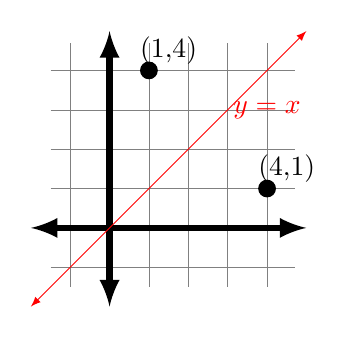
\begin{tikzpicture}[scale=0.5]
        \draw[step=1cm,help lines] (-1.5,-1.5) grid (4.7,4.7);
        \draw[latex-latex, line width=0.08cm] (-2,0) -- (5,0);
        \draw[latex-latex, line width=0.08cm] (0,-2) -- (0,5);
        \draw[latex-latex, color=red, line width=0.01cm] (-2,-2) -- (5,5);
        \node[color=red] at (4,3) {$y=x$};
        \foreach \j/\l in {1/4,4/1}{
            \filldraw [black] (\j,\l) circle [radius=6pt];
            \draw (\j+0.5,\l+0.5) node{(\j,\l)};}
    \end{tikzpicture}
    \caption{Reflexión respecto a la recta $y = x$.}
    \end{figure}
    \end{myproof}
    
    \item $\begin{pmatrix} -2 & 0 \\ 0 & 1 \end{pmatrix}$
    \begin{myproof}
    \textbf{Efecto geométrico:} Estiramiento por $2$ y reflexión respecto al eje $y$ en el eje $x$; el eje $y$ se mantiene igual.

    \textbf{Kernel:} Sólo el vector cero, ya que la matriz es invertible.

    \textbf{Imagen:} Todo $\mathbb{R}^2$.

    \textbf{Rango:} $2$.

    \textbf{Nulidad:} $0$.

    \textbf{Gráfica:}
    \begin{figure}[H]\centering
    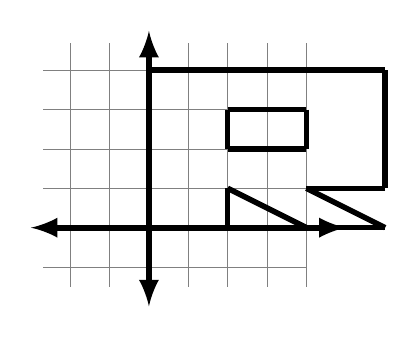
\begin{tikzpicture}[xscale=-0.5,yscale=0.5]
        \draw[step=1cm,help lines] (-4,-1.5) grid (2.7,4.7);
        \draw[latex-latex, line width=0.08cm] (-5,0) -- (3,0);
        \draw[latex-latex, line width=0.08cm] (0,-2) -- (0,5);
        % Dibuja la figura transformada (aproximada)
        \draw [line width=2.pt] (0.,4.)-- (-6.,4.);
        \draw [line width=2.pt] (-6.,4.)-- (-6.,1.);
        \draw [line width=2.pt] (-6.,1.)-- (-4.,1.);
        \draw [line width=2.pt] (-4.,1.)-- (-6.,0.);
        \draw [line width=2.pt] (-4.,0.)-- (-2.,1.);
        \draw [line width=2.pt] (-2.,1.)-- (-2.,0.);
        \draw [line width=2.pt] (-2.,0.)-- (0.,0.);
        \draw [line width=2.pt] (0.,0.)-- (0.,4.);
        \draw [line width=2.pt] (-2.,3.)-- (-4.,3.);
        \draw [line width=2.pt] (-4.,2.)-- (-2.,2.);
        \draw [line width=2.pt] (-2.,2.)-- (-2.,3.);
        \draw [line width=2.pt] (-4.,3.)-- (-4.,2.);
        \draw [line width=2.pt] (-4.,0.)-- (-6.,0.);
    \end{tikzpicture}
    \caption{Estiramiento y reflexión respecto al eje $y$.}
    \end{figure}
    \end{myproof}
    
    \item $\begin{pmatrix} 1 & 0 \\ 0 & 0 \end{pmatrix}$
    \begin{myproof}
    \textbf{Efecto geométrico:} Proyección ortogonal sobre el eje $x$.

    \textbf{Kernel:} Todos los vectores del eje $y$ ($\{(0,y)\}$).

    \textbf{Imagen:} El eje $x$.

    \textbf{Rango:} $1$.

    \textbf{Nulidad:} $1$.

    \textbf{Gráfica:}
    \begin{figure}[H]\centering
    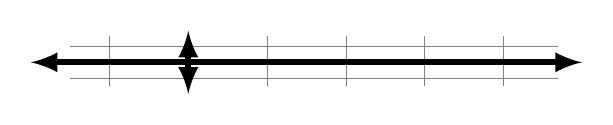
\begin{tikzpicture}[xscale=1,yscale=0.2]
        \draw[step=1cm,help lines] (-1.5,-1.5) grid (4.7,1.7);
        \draw[latex-latex, line width=0.08cm] (-2,0) -- (5,0);
        \draw[latex-latex, line width=0.08cm] (0,-2) -- (0,2);
        % Dibuja la figura proyectada sobre el eje x
        \draw [line width=2.pt] (0.,0.)-- (3.,0.);
    \end{tikzpicture}
    \caption{Proyección sobre el eje $x$.}
    \end{figure}
    \end{myproof}
    
    \item $\begin{pmatrix} 0 & 0 \\ 0 & 1 \end{pmatrix}$
    \begin{myproof}
    \textbf{Efecto geométrico:} Proyección ortogonal sobre el eje $y$.

    \textbf{Kernel:} Todos los vectores del eje $x$ ($\{(x,0)\}$).

    \textbf{Imagen:} El eje $y$.

    \textbf{Rango:} $1$.

    \textbf{Nulidad:} $1$.

    \textbf{Gráfica:}
    \begin{figure}[H]\centering
    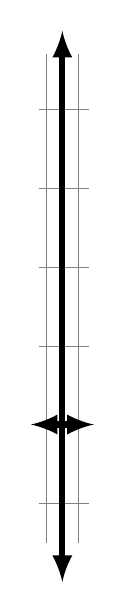
\begin{tikzpicture}[xscale=0.2,yscale=1]
        \draw[step=1cm,help lines] (-1.5,-1.5) grid (1.7,4.7);
        \draw[latex-latex, line width=0.08cm] (-2,0) -- (2,0);
        \draw[latex-latex, line width=0.08cm] (0,-2) -- (0,5);
        % Dibuja la figura proyectada sobre el eje y
        \draw [line width=2.pt] (0.,4.)-- (0.,0.);
    \end{tikzpicture}
    \caption{Proyección sobre el eje $y$.}
    \end{figure}
    \end{myproof}
    
    \item $\begin{pmatrix} 2 & 1 \\ 1 & 3 \end{pmatrix}$
    \begin{myproof}
    \textbf{Efecto geométrico:} Transformación lineal general: estiramiento, cizalladura y rotación.

    \textbf{Kernel:} Sólo el vector cero, ya que el determinante es $2 \cdot 3 - 1 \cdot 1 = 5 \neq 0$.

    \textbf{Imagen:} Todo $\mathbb{R}^2$.

    \textbf{Rango:} $2$.

    \textbf{Nulidad:} $0$.

    \textbf{Gráfica:}
    \begin{figure}[H]\centering
    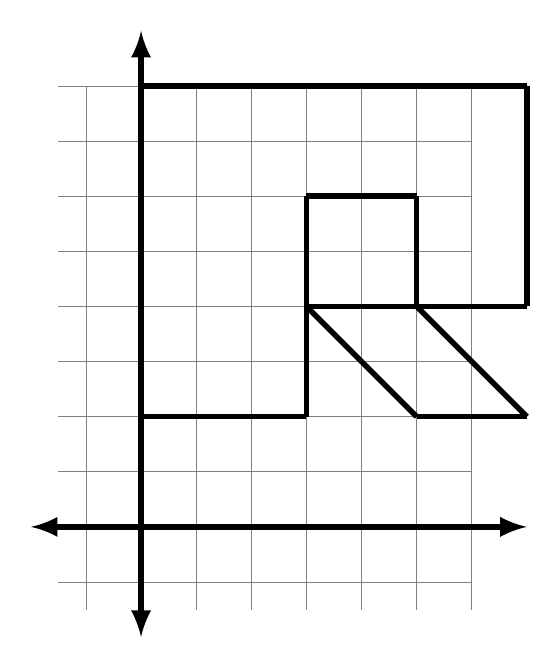
\begin{tikzpicture}[xscale=0.7,yscale=0.7]
        \draw[step=1cm,help lines] (-1.5,-1.5) grid (6,8);
        \draw[latex-latex, line width=0.08cm] (-2,0) -- (7,0);
        \draw[latex-latex, line width=0.08cm] (0,-2) -- (0,9);
        % Dibuja la figura transformada (aproximada)
        \draw [line width=2.pt] (0,8)-- (7,8);
        \draw [line width=2.pt] (7,8)-- (7,4);
        \draw [line width=2.pt] (7,4)-- (5,4);
        \draw [line width=2.pt] (5,4)-- (7,2);
        \draw [line width=2.pt] (5,2)-- (3,4);
        \draw [line width=2.pt] (3,4)-- (3,2);
        \draw [line width=2.pt] (3,2)-- (0,2);
        \draw [line width=2.pt] (0,2)-- (0,8);
        \draw [line width=2.pt] (3,6)-- (5,6);
        \draw [line width=2.pt] (5,4)-- (3,4);
        \draw [line width=2.pt] (3,4)-- (3,6);
        \draw [line width=2.pt] (5,6)-- (5,4);
        \draw [line width=2.pt] (5,2)-- (7,2);
    \end{tikzpicture}
    \caption{Transformación general invertible.}
    \end{figure}
    \end{myproof}
    
    \item $\begin{pmatrix} 2 & 0 \\ 0 & 3 \end{pmatrix}$
    \begin{myproof}
    \textbf{Efecto geométrico:} Escalado: estiramiento por $2$ en el eje $x$ y por $3$ en el eje $y$.

    \textbf{Kernel:} Sólo el vector cero, ya que la matriz es invertible.

    \textbf{Imagen:} Todo $\mathbb{R}^2$.

    \textbf{Rango:} $2$.

    \textbf{Nulidad:} $0$.

    \textbf{Gráfica:}
    \begin{figure}[H]\centering
    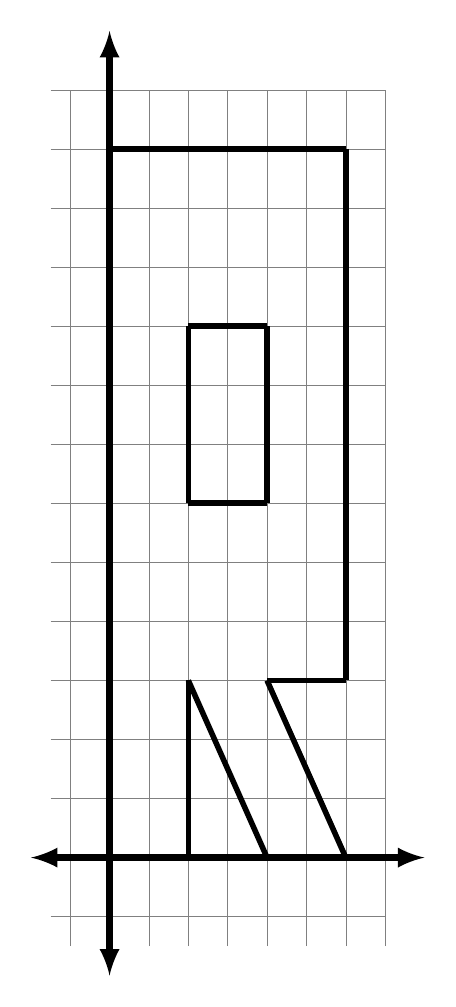
\begin{tikzpicture}[xscale=0.5,yscale=0.75]
        \draw[step=1cm,help lines] (-1.5,-1.5) grid (7,13);
        \draw[latex-latex, line width=0.08cm] (-2,0) -- (8,0);
        \draw[latex-latex, line width=0.08cm] (0,-2) -- (0,14);
        % Dibuja la figura transformada (aproximada)
        \draw [line width=2.pt] (0,12)-- (6,12);
        \draw [line width=2.pt] (6,12)-- (6,3);
        \draw [line width=2.pt] (6,3)-- (4,3);
        \draw [line width=2.pt] (4,3)-- (6,0);
        \draw [line width=2.pt] (4,0)-- (2,3);
        \draw [line width=2.pt] (2,3)-- (2,0);
        \draw [line width=2.pt] (2,0)-- (0,0);
        \draw [line width=2.pt] (0,0)-- (0,12);
        \draw [line width=2.pt] (2,9)-- (4,9);
        \draw [line width=2.pt] (4,6)-- (2,6);
        \draw [line width=2.pt] (2,6)-- (2,9);
        \draw [line width=2.pt] (4,9)-- (4,6);
        \draw [line width=2.pt] (4,0)-- (6,0);
    \end{tikzpicture}
    \caption{Escalado anisotrópico.}
    \end{figure}
    \end{myproof}

    \item $\begin{pmatrix} \cos\left( \frac{\pi}{6} \right) & -\sin\left( \frac{\pi}{6} \right) \\ \sin\left( \frac{\pi}{6} \right) & \cos\left( \frac{\pi}{6} \right) \end{pmatrix}$
    \begin{myproof}
    \textbf{Efecto geométrico:} Rotación antihoraria de $\frac{\pi}{6}$ radianes ($30^\circ$) respecto al origen.

    \textbf{Kernel:} Sólo el vector cero, ya que la matriz de rotación es invertible.

    \textbf{Imagen:} Todo $\mathbb{R}^2$.

    \textbf{Rango:} $2$.

    \textbf{Nulidad:} $0$.

    \textbf{Gráfica:}
    \begin{figure}[H]\centering
    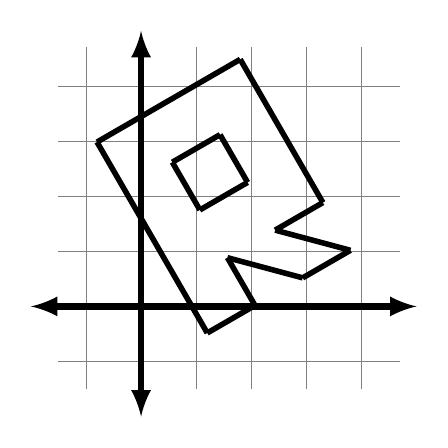
\begin{tikzpicture}[scale=0.7]
        \draw[step=1cm,help lines] (-1.5,-1.5) grid (4.7,4.7);
        \draw[latex-latex, line width=0.08cm] (-2,0) -- (5,0);
        \draw[latex-latex, line width=0.08cm] (0,-2) -- (0,5);
        % Dibuja la figura rotada (aproximada)
        \draw [rotate around={30:(1.5,2)},line width=2.pt] (0.,4.)-- (3.,4.);
        \draw [rotate around={30:(1.5,2)},line width=2.pt] (3.,4.)-- (3.,1.);
        \draw [rotate around={30:(1.5,2)},line width=2.pt] (3.,1.)-- (2.,1.);
        \draw [rotate around={30:(1.5,2)},line width=2.pt] (2.,1.)-- (3.,0.);
        \draw [rotate around={30:(1.5,2)},line width=2.pt] (2.,0.)-- (1.,1.);
        \draw [rotate around={30:(1.5,2)},line width=2.pt] (1.,1.)-- (1.,0.);
        \draw [rotate around={30:(1.5,2)},line width=2.pt] (1.,0.)-- (0.,0.);
        \draw [rotate around={30:(1.5,2)},line width=2.pt] (0.,0.)-- (0.,4.);
        \draw [rotate around={30:(1.5,2)},line width=2.pt] (1.,3.)-- (2.,3.);
        \draw [rotate around={30:(1.5,2)},line width=2.pt] (2.,2.)-- (1.,2.);
        \draw [rotate around={30:(1.5,2)},line width=2.pt] (1.,2.)-- (1.,3.);
        \draw [rotate around={30:(1.5,2)},line width=2.pt] (2.,3.)-- (2.,2.);
        \draw [rotate around={30:(1.5,2)},line width=2.pt] (2.,0.)-- (3.,0.);
    \end{tikzpicture}
    \caption{Rotación de $30^\circ$ respecto al origen.}
    \end{figure}
    \end{myproof}
\end{enumerate}

\end{prob}


\begin{prob}
Dada la siguiente figura tridimensional, determine el efecto geométrico que efectúan sobre ella las transformaciones lineales representadas por las siguientes matrices. Calcule el kernel, la imagen, la nulidad y el rango. Represente gráficamente las transformaciones.

\begin{figure}[H]
\centering 
\begin{tikzpicture}[every node/.style={minimum size=1cm},on grid]
\begin{scope}[every node/.append style={yslant=-0.5},yslant=-0.5]
  \shade[right color=gray!10, left color=black!50] (0,0) rectangle +(3,3);
  \node at (0.5,2.5) {9};
  \node at (1.5,2.5) {7};
  \node at (2.5,2.5) {1};
  \node at (0.5,1.5) {2};
  \node at (1.5,1.5) {4};
  \node at (2.5,1.5) {8};
  \node at (0.5,0.5) {5};
  \node at (1.5,0.5) {3};
  \node at (2.5,0.5) {6};
  \draw (0,0) grid (3,3);
\end{scope}
\begin{scope}[every node/.append style={yslant=0.5},yslant=0.5]
  \shade[right color=gray!70,left color=gray!10] (3,-3) rectangle +(3,3);
  \node at (3.5,-0.5) {3};
  \node at (4.5,-0.5) {9};
  \node at (5.5,-0.5) {7};
  \node at (3.5,-1.5) {6};
  \node at (4.5,-1.5) {1};
  \node at (5.5,-1.5) {5};
  \node at (3.5,-2.5) {8};
  \node at (4.5,-2.5) {2};
  \node at (5.5,-2.5) {4};
  \draw (3,-3) grid (6,0);
\end{scope}
\begin{scope}[every node/.append style={
    yslant=0.5,xslant=-1},yslant=0.5,xslant=-1
  ]
  \shade[bottom color=gray!10, top color=black!80] (6,3) rectangle +(-3,-3);
  \node at (3.5,2.5) {1};
  \node at (3.5,1.5) {4};
  \node at (3.5,0.5) {7};
  \node at (4.5,2.5) {5};
  \node at (4.5,1.5) {6};
  \node at (4.5,0.5) {8};
  \node at (5.5,2.5) {2};
  \node at (5.5,1.5) {3};
  \node at (5.5,0.5) {9};
  \draw (3,0) grid (6,3);
\end{scope}
\end{tikzpicture}
\caption{Figura original (Sudoku 3D cube, \protect\url{https://texample.net/tikz/examples/sudoku-3d-cube})}
\end{figure}

\begin{enumerate}[$a)$]
    \item $\begin{pmatrix} 1 & 0 & 0 \\ 0 & 1 & 0 \\ 0 & 0 & -1 \end{pmatrix}$
    \begin{myproof}
    \textbf{Descripción:} Reflexión respecto al plano $XY$ (cambia el signo de la coordenada $z$).

    \textbf{Kernel:} Sólo el vector cero, pues la matriz es invertible.

    \textbf{Imagen:} Todo $\mathbb{R}^3$.

    \textbf{Rango:} $3$.

    \textbf{Nulidad:} $0$.

    \textbf{Gráfica:}
    \begin{figure}[H]
    \centering
    \begin{tikzpicture}[every node/.style={minimum size=1cm},on grid]
    % Refleja la cara superior a la inferior y viceversa
    \begin{scope}[every node/.append style={yslant=-0.5},yslant=-0.5]
      \shade[right color=gray!10, left color=black!50] (0,0) rectangle +(3,3);
      \node at (0.5,2.5) {9};
      \node at (1.5,2.5) {7};
      \node at (2.5,2.5) {1};
      \node at (0.5,1.5) {2};
      \node at (1.5,1.5) {4};
      \node at (2.5,1.5) {8};
      \node at (0.5,0.5) {5};
      \node at (1.5,0.5) {3};
      \node at (2.5,0.5) {6};
      \draw (0,0) grid (3,3);
    \end{scope}
    \begin{scope}[every node/.append style={yslant=0.5},yslant=0.5]
      \shade[right color=gray!70,left color=gray!10] (3,-3) rectangle +(3,3);
      \node at (3.5,-0.5) {8};
      \node at (4.5,-0.5) {2};
      \node at (5.5,-0.5) {4};
      \node at (3.5,-1.5) {6};
      \node at (4.5,-1.5) {1};
      \node at (5.5,-1.5) {5};
      \node at (3.5,-2.5) {3};
      \node at (4.5,-2.5) {9};
      \node at (5.5,-2.5) {7};
      \draw (3,-3) grid (6,0);
    \end{scope}
    \begin{scope}[every node/.append style={
        yslant=0.5,xslant=-1},yslant=0.5,xslant=-1
      ]
      \shade[bottom color=gray!10, top color=black!80] (6,3) rectangle +(-3,-3);
      \node at (3.5,2.5) {1};
      \node at (3.5,1.5) {4};
      \node at (3.5,0.5) {7};
      \node at (4.5,2.5) {5};
      \node at (4.5,1.5) {6};
      \node at (4.5,0.5) {8};
      \node at (5.5,2.5) {2};
      \node at (5.5,1.5) {3};
      \node at (5.5,0.5) {9};
      \draw (3,0) grid (6,3);
    \end{scope}
    \end{tikzpicture}
    \caption{Reflexión respecto al plano $XY$ (inversión de $z$).}
    \end{figure}
    \end{myproof}
    
    \item $\begin{pmatrix} -5 & 0 & 0 \\ 0 & 1 & 0 \\ 0 & 0 & 3 \end{pmatrix}$
    \begin{myproof}
    \textbf{Descripción:} Escalado anisotrópico: multiplica $x$ por $-5$ (refleja respecto al plano $YZ$ y estira por $5$), deja $y$ igual y multiplica $z$ por $3$ (estiramiento en $z$).

    \textbf{Kernel:} Sólo el vector cero, ya que la matriz es invertible.

    \textbf{Imagen:} Todo $\mathbb{R}^3$.

    \textbf{Rango:} $3$.

    \textbf{Nulidad:} $0$.

    \textbf{Gráfica:}
    \begin{figure}[H]
    \centering
    \begin{tikzpicture}[every node/.style={minimum size=1cm},on grid, xscale=-1.2, yscale=1, yslant=-0.5]
    \shade[right color=gray!10, left color=black!50] (0,0) rectangle +(3,3);
    \node at (0.5,2.5) {9};
    \node at (1.5,2.5) {7};
    \node at (2.5,2.5) {1};
    \node at (0.5,1.5) {2};
    \node at (1.5,1.5) {4};
    \node at (2.5,1.5) {8};
    \node at (0.5,0.5) {5};
    \node at (1.5,0.5) {3};
    \node at (2.5,0.5) {6};
    \draw (0,0) grid (3,3);
    \end{tikzpicture}
    \caption{Reflejo y estiramiento en $x$, estiramiento en $z$.}
    \end{figure}
    \end{myproof}
    
    \item $\begin{pmatrix} 0 & 0 & 0 \\ 1 & 0 & 1 \\ 0 & 0 & 1 \end{pmatrix}$
    \begin{myproof}
    \textbf{Descripción:} Proyección sobre el plano $YZ$ con combinación lineal: la coordenada $x$ se hace cero, $y$ se convierte en $x+z$, $z$ se mantiene.

    \textbf{Kernel:} Todos los vectores de la forma $(a,0,0)$, es decir, el eje $x$.

    \textbf{Imagen:} El plano $YZ$.

    \textbf{Rango:} $2$.

    \textbf{Nulidad:} $1$.

    \textbf{Gráfica:}
    \begin{figure}[H]
    \centering
    \begin{tikzpicture}[every node/.style={minimum size=1cm},on grid, xscale=0.01, yscale=1]
    % Colapsa la figura sobre el plano YZ
    \shade[right color=gray!70,left color=gray!10] (3,-3) rectangle +(3,3);
    \node at (3.5,-0.5) {3};
    \node at (4.5,-0.5) {9};
    \node at (5.5,-0.5) {7};
    \node at (3.5,-1.5) {6};
    \node at (4.5,-1.5) {1};
    \node at (5.5,-1.5) {5};
    \node at (3.5,-2.5) {8};
    \node at (4.5,-2.5) {2};
    \node at (5.5,-2.5) {4};
    \draw (3,-3) grid (6,0);
    \end{tikzpicture}
    \caption{Proyección sobre el plano $YZ$.}
    \end{figure}
    \end{myproof}
    
    \item $\begin{pmatrix} 1 & 0 & 0 \\ 0 & \cos\left( \frac{\pi}{6} \right) & -\sin\left( \frac{\pi}{6} \right) \\ 0 & \sin\left( \frac{\pi}{6} \right) & \cos\left( \frac{\pi}{6} \right) \end{pmatrix}$
    \begin{myproof}
    \textbf{Descripción:} Rotación de $30^\circ$ en el plano $YZ$ alrededor del eje $x$.

    \textbf{Kernel:} Sólo el vector cero, ya que la matriz de rotación es invertible.

    \textbf{Imagen:} Todo $\mathbb{R}^3$.

    \textbf{Rango:} $3$.

    \textbf{Nulidad:} $0$.

    \textbf{Gráfica:}
    \begin{figure}[H]
    \centering
    \begin{tikzpicture}[every node/.style={minimum size=1cm},on grid]
    % La figura se mantiene pero la cara superior e inferior giran en YZ
    \begin{scope}[every node/.append style={yslant=-0.5},yslant=-0.5]
      \shade[right color=gray!10, left color=black!50] (0,0) rectangle +(3,3);
      \node at (0.5,2.5) {9};
      \node at (1.5,2.5) {7};
      \node at (2.5,2.5) {1};
      \node at (0.5,1.5) {2};
      \node at (1.5,1.5) {4};
      \node at (2.5,1.5) {8};
      \node at (0.5,0.5) {5};
      \node at (1.5,0.5) {3};
      \node at (2.5,0.5) {6};
      \draw (0,0) grid (3,3);
    \end{scope}
    \begin{scope}[every node/.append style={yslant=0.5},yslant=0.5, rotate around={-30:(4.5,-1.5)}]
      \shade[right color=gray!70,left color=gray!10] (3,-3) rectangle +(3,3);
      \node at (3.5,-0.5) {3};
      \node at (4.5,-0.5) {9};
      \node at (5.5,-0.5) {7};
      \node at (3.5,-1.5) {6};
      \node at (4.5,-1.5) {1};
      \node at (5.5,-1.5) {5};
      \node at (3.5,-2.5) {8};
      \node at (4.5,-2.5) {2};
      \node at (5.5,-2.5) {4};
      \draw (3,-3) grid (6,0);
    \end{scope}
    \begin{scope}[every node/.append style={
        yslant=0.5,xslant=-1},yslant=0.5,xslant=-1, rotate around={-30:(4.5,1.5)}]
      \shade[bottom color=gray!10, top color=black!80] (6,3) rectangle +(-3,-3);
      \node at (3.5,2.5) {1};
      \node at (3.5,1.5) {4};
      \node at (3.5,0.5) {7};
      \node at (4.5,2.5) {5};
      \node at (4.5,1.5) {6};
      \node at (4.5,0.5) {8};
      \node at (5.5,2.5) {2};
      \node at (5.5,1.5) {3};
      \node at (5.5,0.5) {9};
      \draw (3,0) grid (6,3);
    \end{scope}
    \end{tikzpicture}
    \caption{Rotación de $30^\circ$ en el plano $YZ$ alrededor del eje $x$.}
    \end{figure}
    \end{myproof}
\end{enumerate}
\end{prob}


\begin{prob}
Sea $T: \mathbb{R}^4 \to \mathbb{R}^3$ una transformación lineal definida por $T(\mathbf{x}) = A\mathbf{x}$, donde:
\[
A = \begin{pmatrix} 1 & 2 & 1 & 0 \\ 0 & 1 & 1 & 1 \\ 1 & 3 & 2 & 1 \end{pmatrix}
\]

\begin{enumerate}[(a)]
\item Encuentre una base para $\ker(T)$ y $\operatorname{Im}(T)$.
\begin{myproof}
Para encontrar una base del núcleo (kernel), resolvemos $A\mathbf{x} = 0$:
\[
\ker(T) = \left\{ \begin{pmatrix} x_1 \\ x_2 \\ x_3 \\ x_4 \end{pmatrix} \in \mathbb{R}^4 : 
\begin{pmatrix} 1 & 2 & 1 & 0 \\ 0 & 1 & 1 & 1 \\ 1 & 3 & 2 & 1 \end{pmatrix} 
\begin{pmatrix} x_1 \\ x_2 \\ x_3 \\ x_4 \end{pmatrix} = 0 \right\}
\]
El cálculo computacional muestra que una base de $\ker(T)$ es:
\[
\left\{
\begin{pmatrix} 1 \\ -1 \\ 1 \\ 0 \end{pmatrix},
\begin{pmatrix} 2 \\ -1 \\ 0 \\ 1 \end{pmatrix}
\right\}
\]

Para la imagen (columna espacio), una base está dada por las columnas linealmente independientes de $A$. El cálculo computacional muestra que una base de $\operatorname{Im}(T)$ es:
\[
\left\{
\begin{pmatrix} 1 \\ 0 \\ 1 \end{pmatrix},
\begin{pmatrix} 2 \\ 1 \\ 3 \end{pmatrix}
\right\}
\]
\end{myproof}

\item Verifique el teorema del rango-nulidad para $T$.
\begin{myproof}
El teorema del rango-nulidad establece que:
\[
\operatorname{nulidad}(T) + \operatorname{rango}(T) = \dim(\mathbb{R}^4) = 4
\]
Del inciso anterior, la nulidad es $2$ (dos vectores en la base del núcleo) y el rango es $2$ (dos vectores en la base de la imagen). Por lo tanto:
\[
2 + 2 = 4
\]
El teorema se cumple.
\end{myproof}

\item Determine si $T$ es inyectiva, sobreyectiva o biyectiva.
\begin{myproof}
$T$ es \textbf{inyectiva} si y sólo si el núcleo es trivial, es decir, sólo contiene el vector cero. Como la nulidad es $2$, $T$ \textbf{no es inyectiva}.

$T$ es \textbf{sobreyectiva} si su imagen es todo $\mathbb{R}^3$, es decir, si el rango es $3$. Como el rango es $2$, $T$ \textbf{no es sobreyectiva}.

$T$ es \textbf{biyectiva} si es inyectiva y sobreyectiva. Por lo anterior, $T$ \textbf{no es biyectiva}.
\end{myproof}
\end{enumerate}
\end{prob}
